% ============================================================
%  APUNTES DE CÁTEDRA — AED II y III
%  E.E.S.T. N° 1 — Vicente López
%  Autor: Ariel Wels
% ============================================================
%
% COMPILACIÓN:
%   pdflatex main.tex && pdflatex main.tex
%   (segunda pasada para índice y referencias cruzadas)
%
%   Con latexmk (recomendado, resuelve pasadas automáticamente):
%   latexmk -pdf main.tex
%
%   Para compilar solo un capítulo (más rápido al editar):
%   Descomentar la línea \includeonly{} correspondiente,
%   luego compilar normalmente:
%     \includeonly{capitulo1}    % solo Lógica Secuencial
%     \includeonly{capitulo2}    % solo Memorias
%     \includeonly{capitulo3}    % solo Sistemas Microprogramables
%     \includeonly{capitulo4}    % solo Algoritmos
%     \includeonly{capitulo5}    % solo Introducción a C
%     \includeonly{capitulo6}    % solo C Embebido
%
% ============================================================

\documentclass[a4paper,spanish,12pt]{report}

% --- Fuente y codificación ---
\usepackage{lmodern}
\renewcommand{\familydefault}{\sfdefault}
\usepackage[T1]{fontenc}
\usepackage[utf8]{inputenc}
\usepackage[spanish,es-nodecimaldot,es-noshorthands]{babel}

% --- Geometría de página ---
\usepackage[margin=1in,headsep=1cm,headheight=1.2in,top=1.8in]{geometry}

% --- Matemática ---
\usepackage{amsmath}
\usepackage{amssymb}
\usepackage{mathtools}

% --- Tablas ---
\usepackage{array}
\usepackage{multirow}
\usepackage{booktabs}
\usepackage{tabularx}
\usepackage{longtable}
\usepackage[table]{xcolor}

% --- Gráficos y figuras ---
\usepackage{graphicx}
\usepackage{float}
\usepackage{caption}
\usepackage{subcaption}
\usepackage{pgf,tikz}
\usepackage[siunitx]{circuitikz}
\usetikzlibrary{arrows,arrows.meta,shapes.symbols,shapes.arrows,calc,
                intersections,through,backgrounds,patterns,
                automata,positioning}

% --- Encabezados y pies de página ---
\usepackage{fancyhdr}
\usepackage{lastpage}

% --- Formato de secciones ---
\usepackage{titlesec}

% --- Cajas y notas ---
\usepackage[most]{tcolorbox}
\tcbuselibrary{breakable,skins}

% --- Código fuente ---
\usepackage{listings}
\usepackage{textcomp}

% --- Miscelánea ---
\usepackage{calc}
\usepackage{enumitem}
\usepackage{multicol}
\usepackage{lscape}
\usepackage{rotating}

% --- Hipervínculos (cargar último) ---
\usepackage{tikz-timing}
\usetikztiminglibrary{either}
\usepackage[colorlinks=true,linkcolor=teal!80!black,
            urlcolor=blue!70!black,citecolor=teal]{hyperref}

% ============================================================
%  RUTAS DE IMÁGENES
% ============================================================
\graphicspath{{imagenes/}}

% ============================================================
%  FORMATO DE CAPÍTULOS Y SECCIONES
% ============================================================

% Capítulo: barra teal oscura con número y título
\titleformat{\chapter}[block]
  {\sffamily\bfseries\LARGE}
  {}
  {0pt}
  {\colorchapter}
\titlespacing*{\chapter}{0pt}{0pt}{1.5\baselineskip}

\newcommand{\colorchapter}[1]{%
  \colorbox{teal!70}{%
    \parbox{\dimexpr\textwidth-2\fboxsep}{%
      \strut\color{white}\quad Capítulo \thechapter \quad—\quad #1\strut}}}

% Sección: barra teal media (igual al ejemplo de la institución)
\titleformat{name=\section}[block]
  {\sffamily\bfseries\Large}
  {}
  {0pt}
  {\colorsection}
\titlespacing{\section}{0pt}{\baselineskip}{\baselineskip}

\newcommand{\colorsection}[1]{%
  \colorbox{teal!40}{\parbox{\dimexpr\textwidth-2\fboxsep}{\ #1}}}

% Subsección: barra teal clara
\titleformat{name=\subsection}[block]
  {\sffamily\bfseries\large}
  {}
  {0pt}
  {\colorsubsection}
\titlespacing{\subsection}{0pt}{0.8\baselineskip}{0.5\baselineskip}

\newcommand{\colorsubsection}[1]{%
  \colorbox{teal!20}{\parbox{\dimexpr\textwidth-2\fboxsep}{\ #1}}}

% Subsubsección: texto en negrita sin barra
\titleformat{\subsubsection}[hang]
  {\sffamily\bfseries\normalsize}
  {\thesubsubsection.}{0.5em}{}
\titlespacing{\subsubsection}{0pt}{0.6\baselineskip}{0.3\baselineskip}

% Profundidad de numeración y de TOC
\setcounter{secnumdepth}{3}
\setcounter{tocdepth}{3}

% Marcas para encabezado (sin mayúsculas forzadas)
\renewcommand{\chaptermark}[1]{\markboth{#1}{}}
\renewcommand{\sectionmark}[1]{\markright{#1}}

% ============================================================
%  CÓDIGO FUENTE — LISTINGS  (tema Atom One Light)
% ============================================================

% --- Paleta de colores: Atom One Light ---
\definecolor{atm-bg}{HTML}{FAFAFA}       % fondo (blanco hueso)
\definecolor{atm-fg}{HTML}{383A42}       % texto normal (gris oscuro)
\definecolor{atm-purple}{HTML}{A626A4}   % keywords de control (if, while, return…)
\definecolor{atm-red}{HTML}{E45649}      % tipos primitivos (int, char, void…)
\definecolor{atm-blue}{HTML}{4078F2}     % funciones y registros AVR
\definecolor{atm-green}{HTML}{50A14F}    % strings y char literals
\definecolor{atm-comment}{HTML}{A0A1A7} % comentarios (gris claro)
\definecolor{atm-num}{HTML}{986801}      % literales numéricos (ámbar)
\definecolor{atm-directive}{HTML}{A626A4}% directivas preprocesador (#include)
\definecolor{atm-linenum}{HTML}{C0C0C0} % números de línea
\definecolor{atm-border}{HTML}{DBDBDC}  % borde sutil

% --- Estilo C (Atom One Light) ---
\lstdefinestyle{estilo-c}{
  language=C,
  % Colores base
  backgroundcolor=\color{atm-bg},
  basicstyle=\ttfamily\footnotesize\color{atm-fg},
  % Comentarios: gris claro itálica
  commentstyle=\color{atm-comment}\itshape,
  % Palabras clave: violeta (if, else, while, for, return, switch…)
  % y rojo para tipos (int, char, void, float, double…) — emph clase 1
  keywordstyle=\color{atm-purple},
  % Strings y char literals: verde
  stringstyle=\color{atm-green},
  % Directivas de preprocesador (#include, #define): violeta
  directivestyle=\color{atm-directive},
  % Números de línea: gris claro
  numberstyle=\tiny\color{atm-linenum},
  % Tipos primitivos del C: rojo-naranja (emph clase 1)
  emph={[1]int,char,void,float,double,long,short,unsigned,signed,
        uint8_t,uint16_t,uint32_t,int8_t,int16_t,int32_t,
        size_t,bool,true,false,NULL,FILE},
  emphstyle={[1]\color{atm-red}},
  % Registros, macros e identificadores AVR: azul (emph clase 2)
  emph={[2]ISR,sei,cli,_BV,bit_is_set,bit_is_clear,
        loop_until_bit_is_set,loop_until_bit_is_clear,
        DDRB,DDRC,DDRD,PORTB,PORTC,PORTD,PINB,PINC,PIND,
        TCCR0A,TCCR0B,OCR0A,TIMSK0,TCNT0,TIFR0,
        TIMER0_COMPA_vect,
        OCIE0A,WGM01,WGM00,CS02,CS01,CS00,
        F_CPU},
  emphstyle={[2]\color{atm-blue}},
  % Numeración y espaciado
  numbers=left,
  numbersep=8pt,
  xleftmargin=1.8em,
  % Frame: borde izquierdo fino, sin caja completa
  frame=l,
  framesep=4pt,
  rulecolor=\color{atm-border},
  framerule=1.5pt,
  % Opciones de formato
  breaklines=true,
  breakatwhitespace=false,
  tabsize=4,
  keepspaces=true,
  showspaces=false,
  showstringspaces=false,
  showtabs=false,
  captionpos=b,
}

% --- Estilo pseudocódigo (PSeInt) — misma paleta, sin directivas ---
\lstdefinestyle{estilo-pseudocode}{
  backgroundcolor=\color{atm-bg},
  basicstyle=\ttfamily\footnotesize\color{atm-fg},
  commentstyle=\color{atm-comment}\itshape,
  keywordstyle=\color{atm-purple}\bfseries,
  stringstyle=\color{atm-green},
  numberstyle=\tiny\color{atm-linenum},
  numbers=left,
  numbersep=8pt,
  xleftmargin=1.8em,
  frame=l,
  framesep=4pt,
  framerule=1.5pt,
  rulecolor=\color{atm-border},
  breaklines=true,
  tabsize=4,
  keepspaces=true,
  showstringspaces=false,
}

% --- Aplicar estilo C por defecto + soporte UTF-8 ---
\lstset{
  style=estilo-c,
  literate=
    {á}{{\'{a}}}1 {é}{{\'{e}}}1 {í}{{\'{\i}}}1 {ó}{{\'{o}}}1 {ú}{{\'{u}}}1
    {Á}{{\'{A}}}1 {É}{{\'{E}}}1 {Í}{{\'{I}}}1 {Ó}{{\'{O}}}1 {Ú}{{\'{U}}}1
    {ñ}{{\~{n}}}1 {Ñ}{{\~{N}}}1
    {ü}{{\"u}}1   {Ü}{{\"U}}1
    {—}{{---}}1   {–}{{--}}1
    {°}{{\textdegree}}1
    {²}{{$^2$}}1  {³}{{$^3$}}1
    {¡}{{!`}}1    {¿}{{?`}}1,
}

% ============================================================
%  CAJAS TCOLORBOX
% ============================================================

\newtcolorbox{notabox}{
  enhanced,
  colback=amber!8,
  colframe=orange!60!black,
  boxrule=1pt,
  leftrule=4pt,
  title=\textbf{Nota},
  fonttitle=\sffamily\bfseries\small,
  attach boxed title to top left={xshift=6pt,yshift=-3pt},
  boxed title style={colback=orange!60!black,colframe=orange!60!black},
  breakable,
}

\newtcolorbox{advertenciabox}{
  enhanced,
  colback=red!5,
  colframe=red!60!black,
  boxrule=1pt,
  leftrule=4pt,
  title=\textbf{Atención},
  fonttitle=\sffamily\bfseries\small,
  attach boxed title to top left={xshift=6pt,yshift=-3pt},
  boxed title style={colback=red!60!black,colframe=red!60!black},
  breakable,
}

\newtcolorbox{importantebox}{
  enhanced,
  colback=teal!5,
  colframe=teal!60!black,
  boxrule=1pt,
  leftrule=4pt,
  title=\textbf{Importante},
  fonttitle=\sffamily\bfseries\small,
  attach boxed title to top left={xshift=6pt,yshift=-3pt},
  boxed title style={colback=teal!60!black,colframe=teal!60!black},
  breakable,
}

% Colores predefinidos extra
\colorlet{amber}{yellow!80!red}

% ============================================================
%  INSERCIÓN DE ARCHIVOS .tikz EXTERNOS
%  Uso: \tikzCircuito{nombre-sin-extension}{caption}
%  Si el archivo tikz/<nombre>.tikz existe → lo muestra con banner.
%  Si todavía no existe → cae a \imagenPendiente automáticamente.
% ============================================================
\newcommand{\tikzCircuito}[2]{%
  \IfFileExists{tikz/#1.tikz}{%
    \bannerRevision
    \begin{figure}[H]
    \centering
    \input{tikz/#1.tikz}%
    \caption{#2}%
    \end{figure}%
  }{%
    \imagenPendiente{#2}%
  }%
}

% ============================================================
%  BANNER TEMPORAL — marca diagramas CircuiTikZ para revisar
% ============================================================
\newcommand{\bannerRevision}{%
  \vspace{4pt}%
  \noindent\begin{tcolorbox}[colback=yellow!25,colframe=orange!70!black,
    left=5pt,right=5pt,top=2pt,bottom=2pt,
    boxrule=1pt,arc=2pt]%
    {\sffamily\bfseries\footnotesize\color{orange!80!black}%
     $\blacktriangleright$\ Diagrama generado en CircuiTikZ\ ---
     revisar antes de la versión final}%
  \end{tcolorbox}\vspace{2pt}\noindent}

% ============================================================
%  IMAGEN PENDIENTE (placeholder hasta insertar figuras reales)
% ============================================================
\newcommand{\imagenPendiente}[1]{%
  \begin{figure}[H]
    \centering
    \setlength{\fboxsep}{12pt}
    \fbox{\parbox{0.75\textwidth}{%
      \centering\color{gray!70}%
      \textit{[Imagen pendiente: #1]}}}
    \caption[#1]{#1}
  \end{figure}%
}

% ============================================================
%  ENCABEZADO Y PIE DE PÁGINA
% ============================================================
\pagestyle{fancy}
\fancyhf{}

\lhead{%
  \begin{tikzpicture}[baseline=(current bounding box.center)]
    \node (logo) at (0,0) {
\includegraphics[width=0.5in]{logo}};
    \node [text width=8cm,align=left,xshift=4.5cm] at (0,0) {%
      \textbf{E.E.S.T.\ N$^\circ$\ 1\ ---\ Vte.\ López}\\
      AED\ II\ y\ III\\
      Apuntes de Cátedra};
  \end{tikzpicture}%
}

\rhead{\nouppercase{\leftmark} \\ \nouppercase{\rightmark}}

\renewcommand{\headrulewidth}{2pt}
\renewcommand{\footrulewidth}{1pt}

\rfoot{\thepage\ de \pageref{LastPage}}
\cfoot{%
  \footnotesize
  \textbf{Escuela de Educación Secundaria Técnica N$^\circ$ 1 --- Vicente López}\\
  Cerrito N$^\circ$ 3966 (1605) Villa Adelina, Partido de Vicente López.%
}

% ============================================================
%  DOCUMENTO
% ============================================================
\begin{document}

% --- Portada ---
\begin{titlepage}
  \centering
  \vspace*{1cm}
  {
\includegraphics[width=0.45\textwidth]{logo}\par}
  \vspace{1cm}
  {\bfseries\LARGE
    Escuela de Educación Secundaria Técnica N\(^{\circ}\) 1\\[0.3em]
    de Vicente López --- Eduardo Ader\par}
  \vspace{0.8cm}
  {\large Aplicaciones de Electrónica Digital II y III\quad---\quad 5\(^{\circ}\) Año\par}
  \vspace{3cm}
  {\Huge\bfseries\color{teal!80!black} Apuntes de Cátedra\par}
  \vspace{2cm}
  {\Large Docente: Ariel Wels\par}
  \vfill
  {\large Ciclo Lectivo 2025\par}
\end{titlepage}

% --- Índice ---
\clearpage
\fancyhead{}
\fancyhead[C]{\textbf{ÍNDICE}}
\tableofcontents
\clearpage

% Restaurar encabezado completo después del índice
\fancyhead{}
\lhead{%
  \begin{tikzpicture}[baseline=(current bounding box.center)]
    \node (logo) at (0,0) {
\includegraphics[width=0.5in]{logo}};
    \node [text width=8cm,align=left,xshift=4.5cm] at (0,0) {%
      \textbf{E.E.S.T.\ N$^\circ$\ 1\ ---\ Vte.\ López}\\
      AED\ II\ y\ III\\
      Apuntes de Cátedra};
  \end{tikzpicture}%
}
\rhead{\nouppercase{\leftmark} \\ \nouppercase{\rightmark}}

% ============================================================
%  CAPÍTULOS
%  Para compilar solo un capítulo, descomentar la línea:
%  \includeonly{capitulos/capitulo1}
% ============================================================

\chapter{Lógica Secuencial}

\section{Lógica combinacional vs. lógica secuencial}

En lógica combinacional, las salidas dependen únicamente del valor actual de las entradas. En lógica \textbf{secuencial}, las salidas dependen tanto de las entradas actuales como del \textbf{estado anterior} del circuito. Esto significa que el circuito tiene memoria: recuerda lo que ocurrió antes.

El bloque fundamental de la lógica secuencial es el \textbf{dispositivo biestable}: un circuito que puede permanecer indefinidamente en uno de dos estados estables (SET o RESET), y que solo cambia de estado cuando se lo indica una señal de entrada.

Los dispositivos biestables se dividen en dos categorías:

\begin{itemize}
    \item \textbf{Latches:} cambian de estado de forma asíncrona, es decir, responden directamente al nivel de sus entradas en cualquier momento.
    \item \textbf{Flip-flops:} cambian de estado de forma síncrona, es decir, solo en el momento en que ocurre un flanco de la señal de reloj.
\end{itemize}

\section{Latches}

\subsection{Latch SR (Set-Reset)}

Es el tipo más simple de dispositivo biestable. Tiene dos entradas (S y R) y dos salidas complementarias (Q y $\overline{Q}$).

Puede implementarse con dos puertas NOR (entradas activas a nivel alto) o con dos puertas NAND (entradas activas a nivel bajo).

\begin{figure}[H]
\centering
% ============================================================
%  Latch SR — implementación con compuertas (figura 7.1 Floyd)
%   Izquierda:  con NOR  -> entradas S, R activas en ALTO
%   Derecha:    con NAND -> entradas Sbar, Rbar activas en BAJO
%  Las compuertas están acopladas en CRUZ: la salida de cada una
%  realimenta una entrada de la otra (el lazo de realimentación se
%  dibuja rodeando el par de compuertas).
%
%  LÓGICA (importante): en el latch NOR, S debe poner Q=1. Como el NOR
%  invierte, S entra en la compuerta cuya salida es Qbar (abajo) y R en
%  la de salida Q (arriba). Por eso R queda arriba y S abajo.
%  (En el NAND activo-bajo, Sbar arriba sí produce Q arriba.)
% ============================================================
%  CÓMO AJUSTAR:
%   - Separación vertical de compuertas: el y=±1.2 de cada \node
%   - Separación NOR/NAND:               el shift={(8,0)} del 2º scope
%   - Tamaño del lazo de realimentación: los ++(0,±4) y ++(-5.x,0)
%   NOTA: el único cruce de cable SIN punto (realim. Qbar sobre la
%         línea de Q) NO conecta; el punto (\circ) marca la derivación.
% ============================================================
\begin{circuitikz}[transform shape, scale=0.8]

  % ===================== Latch con NOR (activo en alto) =====================
  \node[ieeestd nor port] (a) at (0, 1.2) {};    % salida Q
  \node[ieeestd nor port] (b) at (0,-1.2) {};    % salida Qbar
  \draw (a.in 1) -- ++(-1.2,0)node[left]{\small $R$};
  \draw (b.in 2) -- ++(-1.2,0)node[left]{\small $S$};
  \draw (a.out) -- ++(0.2,0) coordinate(qa) -- ++(0.6,0) node[right]{\small $Q$}            ;
  \draw (b.out) -- ++(0.2,0) coordinate(qb) -- ++(0.6,0) node[right]{\small $\overline{Q}$} ;
  \node[circ] at (qa){};   
  \node[circ] at (qb){};
  \draw (qa) -- ++(0,-0.5) --++(-2.5,-1) |- (b.in 1);
  \draw (qb) -- ++(0, 0.5) --++(-2.5, 1) |- (a.in 2);


  % ===================== Latch con NAND (activo en bajo) =====================
  \begin{scope}[shift={(8,0)}]
    \node[ieeestd nand port] (c) at (0, 1.2) {};   % salida Q
    \node[ieeestd nand port] (d) at (0,-1.2) {};   % salida Qbar
    \draw (c.in 1) -- ++(-1.2,0)node[left]{\small $\overline{S}$};
    \draw (d.in 2) -- ++(-1.2,0)node[left]{\small $\overline{R}$};
    \draw (c.out) -- ++(0.2,0) coordinate(qc) -- ++(0.6,0) node[right]{\small $Q$}            ;
    \draw (d.out) -- ++(0.2,0) coordinate(qd) -- ++(0.6,0) node[right]{\small $\overline{Q}$} ;
    \node[circ] at (qc){};   
    \node[circ] at (qd){};
    \draw (qc) -- ++(0,-0.5) --++(-2.5,-1) |- (d.in 1);
    \draw (qd) -- ++(0, 0.5) --++(-2.5, 1) |- (c.in 2);
  \end{scope}

\end{circuitikz}

\caption{Latch SR: implementación con puertas NOR (izquierda, entradas activas alto)
  y puertas NAND (derecha, entradas activas bajo).
  Los cruces de cables sin punto indican que los conductores no se conectan.}
\end{figure}

\tikzCircuito{cap1/latch-SR-simbolo}{Símbolo lógico del latch SR: representación en bloque con entradas S, R y salidas Q, $\overline{Q}$ (figura 7.4 Floyd)}

\textbf{Tabla de verdad --- Latch SR (puertas NOR, entradas activas alto):}

\begin{table}[H]
\centering
\begin{tabular}{ccccp{6cm}}
\toprule
$S$ & $R$ & $Q$ & $\overline{Q}$ & Condición \\
\midrule
0 & 0 & $Q_0$ & $\overline{Q_0}$ & No cambia (retiene estado) \\
1 & 0 & 1 & 0 & SET (Q pasa a 1) \\
0 & 1 & 0 & 1 & RESET (Q pasa a 0) \\
1 & 1 & ? & ? & \textbf{No válido} \\
\bottomrule
\end{tabular}
\end{table}

La condición no válida ocurre cuando ambas entradas se activan simultáneamente: fuerza a ambas salidas al mismo nivel, violando la condición de complementariedad. Si luego se desactivan al mismo tiempo, el estado final es impredecible.

\bannerRevision
\begin{figure}[H]
\centering
\begin{tikztimingtable}[
  timing/slope=0,
  timing/coldist=2pt,
  timing/rowdist=3.8ex,
  timing/name/.style={font=\small\sffamily, right},
  xscale=0.9
]
  $S$            & 2L 2H 8L \\
  $R$            & 8L 2H 2L \\
  $Q$            & 2X 6H 4L \\
  $\overline{Q}$ & 2X 6L 4H \\
  \extracode
    % líneas de referencia en las transiciones
    \begin{pgfonlayer}{background}
      \draw[lightgray, dashed] (2,0.4) -- (2,-5.2);
      \draw[lightgray, dashed] (4,0.4) -- (4,-5.2);
      \draw[lightgray, dashed] (8,0.4) -- (8,-5.2);
      \draw[lightgray, dashed] (10,0.4) -- (10,-5.2);
    \end{pgfonlayer}
    % etiquetas de fase (encima de la primera señal)
    \node[font=\footnotesize\sffamily,above] at (1, 0.4)  {Hold};
    \node[font=\footnotesize\sffamily,above] at (3, 0.4)  {SET};
    \node[font=\footnotesize\sffamily,above] at (6, 0.4)  {Hold};
    \node[font=\footnotesize\sffamily,above] at (9, 0.4)  {RESET};
    \node[font=\footnotesize\sffamily,above] at (11,0.4)  {Hold};
\end{tikztimingtable}

\caption{Diagrama de tiempos del latch SR (puertas NOR, entradas activas alto).
  La franja \textit{Hold} indica que el estado se retiene sin cambios.}
\end{figure}

\textbf{Aplicación --- Eliminación de rebote de pulsadores:}

\subsubsection*{¿Qué es el rebote de los contactos?}

Cuando se presiona un pulsador o se acciona un interruptor mecánico, uno esperaría que la señal eléctrica pasara limpiamente de 0 a 1 en un único instante. Sin embargo, los contactos metálicos son físicamente elásticos: al cerrarse, rebotan varias veces antes de quedar en contacto estable. Lo mismo ocurre al abrir el circuito.

Este fenómeno se llama \textbf{rebote de contactos} (\textit{contact bounce} o \textit{switch bounce}). La duración del rebote depende del tipo de pulsador y de su estado mecánico, pero típicamente está entre \textbf{1\,ms y 20\,ms}.

\tikzCircuito{cap1/bounce-signal}{Señal ideal (flanco limpio) vs.\ señal real con rebote (múltiples pulsos breves en la zona de transición)}

\subsubsection*{¿Qué ve el circuito digital durante el rebote?}

Para la electrónica digital no existe el concepto de ``está rebotando'': cada transición de tensión es leída como un cambio de estado válido. Así, un único pulso de dedo puede generar \textbf{5, 10 o más pulsos eléctricos} en los primeros milisegundos. La señal real se ve como una ráfaga de pulsos muy cortos, seguida por un nivel estable. Desde el punto de vista del circuito, esos pulsos son completamente válidos e indistinguibles de pulsaciones reales del usuario.

\subsubsection*{Problemas que genera el rebote}

\begin{table}[H]
\centering
\begin{tabular}{p{5.5cm} p{7cm}}
\toprule
\textbf{Situación} & \textbf{Consecuencia del rebote} \\
\midrule
Contador incrementado por botón & Un solo toque incrementa el contador en 3, 7 u otro número imprevisible \\
\addlinespace
Interrupción por flanco en microcontrolador & La ISR se ejecuta múltiples veces por una única pulsación \\
\addlinespace
Latch o flip-flop activado por botón & El estado puede cambiar varias veces antes de estabilizarse \\
\addlinespace
Sistema de navegación de menú & Un toque avanza varios ítems en lugar de uno \\
\bottomrule
\end{tabular}
\caption{Problemas típicos causados por el rebote de contactos en sistemas digitales.}
\end{table}

El rebote es especialmente problemático con señales de reloj o con pines de interrupción, donde el sistema es sensible a cada flanco individualmente.

\subsubsection*{Solución con latch SR}

Un latch SR puede eliminar el rebote mecánico usando un interruptor SPDT (\textit{Single Pole Double Throw}) conectado entre masa y las entradas $\overline{S}$ y $\overline{R}$ del latch, con resistencias pull-up a Vcc.

Al cambiar la posición del interruptor, el primer contacto activa el latch de forma definitiva. Cualquier rebote posterior aplica la misma entrada (S o R) que ya fue procesada, por lo que \textbf{el estado del latch no vuelve a cambiar}. La salida Q presenta una transición limpia y única.

\tikzCircuito{cap1/debounce-latch}{Circuito eliminador de rebote de pulsadores con latch SR (figura 7.6 Floyd)}

\tikzCircuito{cap1/debounce-timing}{Diagrama de tiempos del circuito antirrebote: señal con rebote en la entrada vs.\ salida Q limpia del latch (figura 7.7 Floyd)}

\subsection{Latch SR con habilitación}

Agrega una entrada de habilitación (EN). El latch solo puede cambiar de estado cuando EN está activo. Permite controlar exactamente en qué momento el latch responde a sus entradas.

\tikzCircuito{cap1/latch-SR-EN}{Diagrama y símbolo del latch SR con habilitación (EN) (figura 7.8 Floyd)}

\textbf{Tabla de verdad --- Latch SR con habilitación (puertas NOR, entradas activas alto):}

\begin{table}[H]
\centering
\begin{tabular}{ccccp{6.5cm}}
\toprule
$S$ & $R$ & EN & $Q$ & Condición \\
\midrule
0 & 0 & 1 & $Q_0$ & No cambia \\
1 & 0 & 1 & 1     & SET (Q pasa a 1) \\
0 & 1 & 1 & 0     & RESET (Q pasa a 0) \\
1 & 1 & 1 & ?     & \textbf{No válido} \\
X & X & 0 & $Q_0$ & No cambia (EN inactivo, S y R ignoradas) \\
\bottomrule
\end{tabular}
\end{table}

\bannerRevision
\begin{figure}[H]
\centering
\begin{tikztimingtable}[
  timing/slope=0,
  timing/coldist=2pt,
  timing/rowdist=3.8ex,
  timing/name/.style={font=\small\sffamily, right},
  xscale=0.9
]
  EN  & 4H 4L 4H \\
  $S$ & 2L 2H 8L \\
  $R$ & 5L 5H 2L \\
  $Q$ & 2L 6H 4L \\
  \extracode
    \begin{pgfonlayer}{background}
      \draw[lightgray, dashed] (2, 0.4) -- (2,-5.2);
      \draw[lightgray, dashed] (4, 0.4) -- (4,-5.2);
      \draw[lightgray, dashed] (5, 0.4) -- (5,-5.2);
      \draw[lightgray, dashed] (8, 0.4) -- (8,-5.2);
      \draw[lightgray, dashed] (10,0.4) -- (10,-5.2);
    \end{pgfonlayer}
    \node[font=\footnotesize\sffamily,above] at (1,  0.4) {Hold};
    \node[font=\footnotesize\sffamily,above] at (3,  0.4) {SET};
    \node[font=\footnotesize\sffamily,above] at (6.5,0.4) {EN=0 (bloqueado)};
    \node[font=\footnotesize\sffamily,above] at (9,  0.4) {RESET};
    \node[font=\footnotesize\sffamily,above] at (11, 0.4) {Hold};
    \node[font=\footnotesize\itshape, anchor=west] at (0,-6.3)
      {R se activa en $t{=}5$ pero es ignorado hasta que EN vuelve a 1 (en $t{=}8$).};
\end{tikztimingtable}

\caption{Diagrama de tiempos del latch SR con habilitación. EN=0 bloquea las entradas:
  aunque R se active mientras EN=0, Q no cambia. El RESET recién ocurre
  cuando EN regresa a 1 (y R sigue activo).}
\end{figure}

\subsection{Latch D con habilitación}

Tiene una única entrada de datos (D) además de la habilitación (EN). Elimina la condición no válida del latch SR: cuando EN está activo, la salida Q sigue al valor de D. Cuando EN se desactiva, el latch retiene el último valor de D.

\tikzCircuito{cap1/latch-D}{Diagrama y símbolo del latch D con habilitación (figura 7.10 Floyd)}

\begin{table}[H]
\centering
\begin{tabular}{ccp{2cm}l}
\toprule
D & EN & Q & Condición \\
\midrule
0 & 1 & 0 & RESET \\
1 & 1 & 1 & SET \\
X & 0 & $Q_0$ & No cambia \\
\bottomrule
\end{tabular}
\end{table}

\bannerRevision
\begin{figure}[H]
\centering
\begin{tikztimingtable}[
  timing/slope=0,
  timing/coldist=2pt,
  timing/rowdist=3.8ex,
  timing/name/.style={font=\small\sffamily, right},
  xscale=0.9
]
  EN  & 4H 4L 4H \\
  $D$ & 2L 2H 2H 2L 2L 2H \\
  $Q$ & 2L 6H 2L 2H \\
  \extracode
    \begin{pgfonlayer}{background}
      % Zona EN=0 sombreada
      \fill[yellow!12] (4,-0.5) rectangle (8,-4.2);
      \draw[lightgray, dashed] (2, 0.4) -- (2,-4.2);
      \draw[lightgray, dashed] (4, 0.4) -- (4,-4.2);
      \draw[lightgray, dashed] (6, 0.4) -- (6,-4.2);
      \draw[lightgray, dashed] (8, 0.4) -- (8,-4.2);
      \draw[lightgray, dashed] (10,0.4) -- (10,-4.2);
    \end{pgfonlayer}
    \node[font=\footnotesize\sffamily,above] at (1, 0.4) {Q=D};
    \node[font=\footnotesize\sffamily,above] at (3, 0.4) {Q=D};
    \node[font=\footnotesize\sffamily,above] at (6, 0.4) {EN=0: Q retiene};
    \node[font=\footnotesize\sffamily,above] at (9, 0.4) {Q=D};
    \node[font=\footnotesize\sffamily,above] at (11,0.4) {Q=D};
    % Destacar cambio de D ignorado
    \node[font=\tiny\itshape, teal!70!black] at (7,-4.8)
      {D cambia a 0 pero Q no cambia (EN=0)};
\end{tikztimingtable}

\caption{Diagrama de tiempos del latch D. Con EN=1 la salida es \textit{transparente}:
  Q sigue inmediatamente a D. Con EN=0 el latch queda \textit{opaco}: retiene el
  último valor de D aunque la entrada cambie (zona sombreada; ver $t{=}6$).}
\end{figure}

\section{Flip-flops}

La diferencia fundamental entre un latch y un flip-flop es el mecanismo de disparo. Un flip-flop \textbf{disparado por flanco} solo cambia de estado en el instante exacto del flanco (de subida o de bajada) de la señal de reloj. Fuera de ese instante, es insensible a los cambios en sus entradas.

En los símbolos lógicos, el flanco activo se indica con un \textbf{triángulo} en la entrada de reloj (indicador de entrada dinámica). Si hay un círculo adicional, el disparo es por flanco negativo (bajada); sin círculo, por flanco positivo (subida).

\bannerRevision
\begin{figure}[H]
\centering
% ============================================================
%  Símbolos de flip-flops disparados por flanco
%  - FF-D flanco ↑ : cuña (triángulo) en la entrada de reloj.
%  - FF-D flanco ↓ : cuña + BURBUJA (círculo de negación) en el reloj.
%  - FF-JK flanco ↑: J, CLK, K.
%  Los FF de circuitikz se definen con "flipflop def" (manual §4.23):
%    tN = texto del pin N, cN=1 dibuja la cuña de reloj,
%    nN=1 dibuja la burbuja de negación en el pin N.
%  Pines: 1,2,3 a la izquierda (arriba→abajo); 6,5,4 a la derecha.
% ============================================================
%  CÓMO AJUSTAR:
%   - Separación entre símbolos: la x de cada \node (0, 5.4, 10.8)
%   - Largo de los cables de entrada/salida: el 0.6 de los ++(...)
%   - Tamaño general: scale= en \begin{circuitikz}
% ============================================================
\begin{circuitikz}[scale=0.85, transform shape,
  flipflop Dn/.style={flipflop,
    flipflop def={t1=D, t6=Q, c3=1, n3=1, t4={\ctikztextnot{Q}}}},
]

  % --- FF-D flanco positivo ---
  \node[flipflop D] (ffd) at (0,0) {};
  \draw (ffd.pin 1) -- ++(-0.6,0) node[left]{\small D};
  \draw (ffd.pin 3) -- ++(-0.6,0) node[left]{\small CLK};
  \draw (ffd.pin 6) -- ++(0.6,0) node[right]{\small $Q$};
  \draw (ffd.pin 4) -- ++(0.6,0) node[right]{\small $\overline{Q}$};
  \node[below=0.35 of ffd.south, font=\small] {Flanco $\uparrow$};

  % --- FF-D flanco negativo (burbuja en CLK) ---
  \node[flipflop Dn] (ffdn) at (5.4,0) {};
  \draw (ffdn.pin 1) -- ++(-0.6,0) node[left]{\small D};
  \draw (ffdn.pin 3) -- ++(-0.6,0) node[left]{\small CLK};
  \draw (ffdn.pin 6) -- ++(0.6,0) node[right]{\small $Q$};
  \draw (ffdn.pin 4) -- ++(0.6,0) node[right]{\small $\overline{Q}$};
  \node[below=0.35 of ffdn.south, font=\small] {Flanco $\downarrow$};

  % --- FF-JK flanco positivo ---
  \node[flipflop JK] (ffjk) at (10.8,0) {};
  \draw (ffjk.pin 1) -- ++(-0.6,0) node[left]{\small J};
  \draw (ffjk.pin 2) -- ++(-0.6,0) node[left]{\small CLK};
  \draw (ffjk.pin 3) -- ++(-0.6,0) node[left]{\small K};
  \draw (ffjk.pin 6) -- ++(0.6,0) node[right]{\small $Q$};
  \draw (ffjk.pin 4) -- ++(0.6,0) node[right]{\small $\overline{Q}$};
  \node[below=0.35 of ffjk.south, font=\small] {Flanco $\uparrow$};

\end{circuitikz}

\caption{Símbolos de flip-flops disparados por flanco. El triángulo en CLK indica
  disparo por flanco; el círculo adicional (centro) indica flanco negativo.}
\end{figure}

\subsection{Flip-flop SR disparado por flanco}

Similar al latch SR pero sincronizado con el reloj. Las entradas S y R solo son evaluadas en el flanco activo del reloj.

\begin{table}[H]
\centering
\begin{tabular}{cccc}
\toprule
S & R & Q siguiente & Condición \\
\midrule
0 & 0 & $Q_0$ & No cambia \\
1 & 0 & 1 & SET \\
0 & 1 & 0 & RESET \\
1 & 1 & ? & No válido \\
\bottomrule
\end{tabular}
\end{table}

\bannerRevision
\begin{figure}[H]
\centering
% ============================================================
%  Flip-flop SR disparado por flanco ascendente: diagrama de tiempos
%  - Las entradas S y R sólo se miran en los flancos ↑ de CLK
%    (t = 1, 3, 5, 7, 9). Entre flancos, Q no cambia.
%  - S y R cambian entre flancos (t par) para no violar setup/hold.
%  Coordenadas: ver tikz/estilos.tex (1 carácter = 1 unidad en x).
% ============================================================
\begin{tikztimingtable}[timing/aed]
  CLK & LHLHLHLHLH \\
  $S$ & 2L 2H 6L \\
  $R$ & 6L 2H 2L \\
  $Q$ & 3L 4H 3L \\
  \extracode
    \begin{pgfonlayer}{background}
      \vertlines{1,3,...,9}
    \end{pgfonlayer}
    \foreach \x/\op in {1/Hold, 3/SET, 5/Hold, 7/RESET, 9/Hold}
      \node[fase] at (\x,1.5) {\op};
\end{tikztimingtable}

\caption{Diagrama de tiempos del flip-flop SR disparado por flanco positivo.
  S y R solo son evaluadas en el flanco de subida del reloj; fuera de ese instante
  los cambios en las entradas no tienen efecto.}
\end{figure}

\subsection{Flip-flop D disparado por flanco}

La salida Q toma el valor de la entrada D en cada flanco activo del reloj. Es el más simple y el más utilizado en la práctica.

\begin{table}[H]
\centering
\begin{tabular}{cc}
\toprule
D & Q siguiente \\
\midrule
0 & 0 \\
1 & 1 \\
\bottomrule
\end{tabular}
\end{table}

\bannerRevision
\begin{figure}[H]
\centering
% ============================================================
%  Flip-flop D disparado por flanco ascendente: diagrama de tiempos
%  - Q copia el valor de D SÓLO en los flancos ↑ de CLK (t = 1,3,5,7,9).
%  - D cambia siempre entre flancos (t par) para no violar setup/hold.
%  Coordenadas: ver tikz/estilos.tex (1 carácter = 1 unidad en x).
% ============================================================
\begin{tikztimingtable}[timing/aed]
  CLK & LHLHLHLHLH \\
  $D$ & 4H 4L 2H   \\
  $Q$ & X 4H 4L H  \\
  \extracode
    \begin{pgfonlayer}{background}
      \vertlines{1,3,...,9}
    \end{pgfonlayer}
    % marca de captura en cada flanco activo
    \foreach \x in {1,3,...,9}
      \node[fase] at (\x,1.5) {$\uparrow$};
    \node[nota] at (0,{-2*\rowdist-1.1})
      {Q copia el valor de D sólo en cada flanco $\uparrow$ de CLK.};
\end{tikztimingtable}

\caption{Diagrama de tiempos del flip-flop D disparado por flanco positivo.
  Cada flanco de subida del reloj transfiere el valor de D a la salida Q.}
\end{figure}

\subsection{Flip-flop JK disparado por flanco}

El flip-flop JK resuelve la condición no válida del SR reemplazando el estado indeterminado por una operación de \textbf{basculación (toggle)}: cuando J = K = 1, la salida cambia de estado en cada flanco de reloj.

\begin{table}[H]
\centering
\begin{tabular}{cccc}
\toprule
J & K & Q siguiente & Condición \\
\midrule
0 & 0 & $Q_0$ & No cambia \\
1 & 0 & 1 & SET \\
0 & 1 & 0 & RESET \\
1 & 1 & $\overline{Q_0}$ & Bascula (Toggle) \\
\bottomrule
\end{tabular}
\end{table}

\tikzCircuito{cap1/flipflop-JK}{Símbolo del flip-flop JK disparado por flanco (figura 7.22 Floyd)}

\subsection{Flip-flop T (Toggle)}

Es un caso especial del JK con ambas entradas unidas (J = K = T). Cuando T = 1, la salida bascula en cada flanco de reloj. Cuando T = 0, la salida no cambia.

\begin{table}[H]
\centering
\begin{tabular}{cc}
\toprule
T & Q siguiente \\
\midrule
0 & $Q_0$ \\
1 & $\overline{Q_0}$ \\
\bottomrule
\end{tabular}
\end{table}

\bannerRevision
\begin{figure}[H]
\centering
% ============================================================
%  Flip-flop T disparado por flanco ascendente: diagrama de tiempos
%  - T=1 en el flanco ↑: Q se invierte (Toggle).
%  - T=0 en el flanco ↑: Q se mantiene (Hold).
%  - Flancos activos en t = 1, 3, 5, 7, 9.
%  Coordenadas: ver tikz/estilos.tex (1 carácter = 1 unidad en x).
% ============================================================
\begin{tikztimingtable}[timing/aed]
  CLK & LHLHLHLHLH \\
  $T$ & 2L 6H 2L \\
  $Q$ & 3L 2H 2L 3H \\
  \extracode
    \begin{pgfonlayer}{background}
      \vertlines{1,3,...,9}
    \end{pgfonlayer}
    \foreach \x/\op in {1/Hold, 3/Toggle, 5/Toggle, 7/Toggle, 9/Hold}
      \node[fase] at (\x,1.5) {\op};
\end{tikztimingtable}

\caption{Diagrama de tiempos del flip-flop T. Con T=0 la salida no cambia
  en el flanco activo; con T=1 la salida bascula en cada flanco de subida,
  dividiendo la frecuencia del reloj por 2.}
\end{figure}

El flip-flop T es la base de los contadores binarios.

\subsection{Entradas asíncronas: Preset y Clear}

La mayoría de los flip-flops tienen entradas asíncronas que actúan \textbf{independientemente del reloj}:

\begin{itemize}
    \item \textbf{Preset (PRE):} fuerza la salida Q a 1.
    \item \textbf{Clear (CLR):} fuerza la salida Q a 0.
\end{itemize}

Son útiles para inicializar el sistema a un estado conocido al encender, o para hacer resets de emergencia.

\subsection{Características de funcionamiento}

Algunas características importantes de los flip-flops al trabajar con señales reales:

\textbf{Retardo de propagación ($t_{pd}$):} tiempo que transcurre desde el flanco activo del reloj hasta que la salida estabiliza su nuevo valor. Limita la frecuencia máxima de operación.

\textbf{Tiempo de establecimiento ($t_{setup}$):} tiempo mínimo que la entrada debe estar estable \textbf{antes} del flanco activo del reloj para garantizar una lectura correcta.

\textbf{Tiempo de mantenimiento ($t_{hold}$):} tiempo mínimo que la entrada debe permanecer estable \textbf{después} del flanco activo del reloj.

\textbf{Frecuencia máxima ($f_{max}$):} frecuencia de reloj máxima a la que el flip-flop puede operar correctamente.

\bannerRevision
\begin{figure}[H]
\centering
\begin{tikzpicture}[
  >=Stealth,
  sig/.style={thick},
  dim/.style={<->,>=Stealth,teal!70!black,thick},
  anno/.style={font=\small\sffamily,teal!80!black},
  lbl/.style={font=\footnotesize\sffamily},
]
  % --- Parámetros de tiempo (unidades arbitrarias) ---
  \def\Tsetup{1.5}   % duración t_setup
  \def\Tclkedge{4}   % posición del flanco de CLK
  \def\Thold{1.5}    % duración t_hold
  \def\Tpd{1.8}      % retardo de propagación (CLK→Q válido)
  \def\Tend{8}

  % --- CLK ---
  \draw[sig] (0,2) -- (\Tclkedge-0.1,2)
             -- (\Tclkedge,3) -- (\Tend,3);   % flanco de subida en \Tclkedge
  \node[lbl,left] at (0,2.5) {CLK};

  % --- D (estable alrededor del flanco) ---
  % D=H antes y después del flanco
  \draw[sig] (0,0.8) -- (1.0,0.8)                  % inicio con dato previo (L)
             -- (1.0,0) -- (\Tclkedge-\Tsetup,0)   % transición de D
             -- (\Tclkedge-\Tsetup,0.8)             % D estable = H desde t_setup antes
             -- (\Tclkedge+\Thold,0.8)          % D estable hasta después de t_hold
             -- (\Tclkedge+\Thold,0)            % D puede cambiar
             -- (\Tend,0);
  \node[lbl,left] at (0,0.4) {D};

  % zona estable de D (relleno, detrás de las señales)
  \begin{pgfonlayer}{background}
    \fill[teal!12] (\Tclkedge-\Tsetup,0) rectangle (\Tclkedge+\Thold,0.8);
  \end{pgfonlayer}

  % --- Q ---
  \draw[sig] (0,-1.2) -- (\Tclkedge+\Tpd,-1.2)  % Q mantiene valor anterior
             -- (\Tclkedge+\Tpd,-0.4)             % Q cambia al nuevo valor
             -- (\Tend,-0.4);
  \node[lbl,left] at (0,-0.8) {Q};
  % zona de propagación (Q no válido)
  \begin{pgfonlayer}{background}
    \fill[orange!15] (\Tclkedge,-1.2) rectangle (\Tclkedge+\Tpd,-0.4);
  \end{pgfonlayer}
  \draw[orange!60,dashed] (\Tclkedge,-1.3) -- (\Tclkedge+\Tpd,-1.3);

  % --- Línea del flanco de CLK ---
  \draw[gray,dashed,thin] (\Tclkedge,-1.5) -- (\Tclkedge,3.5);

  % --- Cotas ---
  % t_setup
  \draw[dim] (\Tclkedge-\Tsetup,1.5) -- (\Tclkedge,1.5)
    node[midway,above,anno]{$t_{setup}$};

  % t_hold
  \draw[dim] (\Tclkedge,1.5) -- (\Tclkedge+\Thold,1.5)
    node[midway,above,anno]{$t_{hold}$};

  % t_pd
  \draw[dim] (\Tclkedge,-1.8) -- (\Tclkedge+\Tpd,-1.8)
    node[midway,below,anno]{$t_{pd}$};

  % flanco de subida
  \draw[->,gray] (\Tclkedge+0.3,2.4) node[right,lbl]{flanco activo} -- (\Tclkedge+0.05,2.8);

\end{tikzpicture}

\caption{Parámetros temporales de un flip-flop: $t_{setup}$ (D debe estar estable antes del flanco),
  $t_{hold}$ (D debe mantenerse estable después del flanco),
  $t_{pd}$ (tiempo desde el flanco hasta que Q es válido).
  La zona sombreada en D indica la ventana de estabilidad requerida.}
\end{figure}

\section{Registros de desplazamiento}

Un registro de desplazamiento es un circuito formado por flip-flops en cascada que cumple dos funciones: \textbf{almacenamiento} y \textbf{desplazamiento} de datos. Cada flip-flop representa un bit; por lo tanto, un registro de N etapas almacena N bits.

Los datos pueden entrar y salir del registro de distintas formas:

\imagenPendiente{los 7 modos básicos de movimiento de datos en un registro (figura 9.2 Floyd)}

\subsection{Entrada serie / Salida serie (SISO)}

Los bits entran uno a uno por un extremo y salen uno a uno por el otro. En cada pulso de reloj, todos los bits se desplazan una posición. Se necesitan N pulsos para cargar N bits y otros N para extraerlos.

\tikzCircuito{cap1/registro-SISO}{Registro de desplazamiento SISO de 4 bits: flip-flops D en cascada (figura 9.3 Floyd)}

\begin{notabox}
\textbf{CI típico:} \textbf{74HC164} --- registro SIPO de 8 bits (serie in / paralelo out). También puede usarse como SISO tomando solo la salida del último flip-flop.
\end{notabox}

\subsection{Entrada serie / Salida paralelo (SIPO)}

Los bits entran en serie pero se leen simultáneamente de todas las salidas Q de cada etapa. Una vez cargados los N bits, están disponibles todos al mismo tiempo en las salidas paralelo. Se usa para convertir datos serie a paralelo, por ejemplo para controlar múltiples LEDs o segmentos usando solo unos pocos pines del microcontrolador.

\begin{notabox}
\textbf{CI típicos:}
\begin{itemize}
    \item \textbf{74HC595} --- registro SIPO de 8 bits con latch de salida separado y salida en colector abierto para cascada. Es el más utilizado en proyectos con microcontroladores para expandir salidas digitales.
    \item \textbf{74HC164} --- registro SIPO de 8 bits sin latch de salida (las salidas cambian mientras se desplazan los datos).
\end{itemize}
\end{notabox}

\imagenPendiente{diagrama de pines y conexión del 74HC595 en cascada con microcontrolador}

\subsection{Entrada paralelo / Salida serie (PISO)}

Los N bits se cargan simultáneamente en las etapas (carga paralelo) y luego se extraen uno a uno en serie. Se usa para convertir datos paralelo a serie, por ejemplo para leer el estado de múltiples entradas digitales usando pocos pines del microcontrolador.

\begin{notabox}
\textbf{CI típicos:}
\begin{itemize}
    \item \textbf{74HC165} --- registro PISO de 8 bits con carga paralela asíncrona. Muy usado para leer matrices de pulsadores o DIP switches desde un microcontrolador por SPI.
    \item \textbf{74LS165} --- versión TTL del mismo.
\end{itemize}
\end{notabox}

\subsection{Entrada paralelo / Salida paralelo (PIPO)}

Los datos se cargan y se leen en paralelo. Funciona esencialmente como un banco de flip-flops D con habilitación. Se usa principalmente como registro de almacenamiento temporal o buffer de datos.

\begin{notabox}
\textbf{CI típico:} \textbf{74HC195} --- registro PIPO de 4 bits con entrada serie y paralelo y salida paralelo.
\end{notabox}

\subsection{Registros bidireccionales}

Pueden desplazar datos tanto hacia la izquierda como hacia la derecha, según el valor de una entrada de control de dirección. Son los más versátiles ya que combinan múltiples modos de operación.

\begin{notabox}
\textbf{CI típicos:}
\begin{itemize}
    \item \textbf{74HC194} --- registro universal de 4 bits: SISO izquierda, SISO derecha, carga paralelo, retención. Controlado por dos entradas de modo (S0, S1).
    \item \textbf{74LS194} --- versión TTL del mismo.
\end{itemize}
\end{notabox}

\subsection{Contadores basados en registros de desplazamiento}

Conectando la salida del último flip-flop a la entrada del primero (registro en anillo), se obtienen secuencias especiales:

\textbf{Contador en anillo:} desplaza un único bit activo de forma circular. Un registro de N etapas genera una secuencia de N estados únicos y requiere N flip-flops para contar N estados (sin decodificador adicional).

\textbf{Contador Johnson (o de anillo torcido):} la salida complementada del último flip-flop ($\overline{Q}$) se realimenta a la entrada del primero. Un registro de N etapas genera una secuencia de 2N estados.

\section{Contadores}

Un contador es un circuito secuencial formado por flip-flops que recorre una secuencia determinada de estados binarios, uno por cada pulso de reloj. El \textbf{módulo} de un contador es la cantidad total de estados distintos que recorre antes de repetirse.

$$\text{Módulo} = 2^N \quad \text{(para un contador binario de N flip-flops)}$$

\subsection{Contadores asíncronos (con propagación)}

El reloj se aplica solo al primer flip-flop. Cada flip-flop siguiente se dispara con la salida del anterior. Los cambios de estado se propagan de etapa en etapa, por eso también se los llama \textbf{contadores con propagación} (\textit{ripple counters}).

\tikzCircuito{cap1/contador-asincrono-4bit}{Contador asíncrono (ripple) de 4 bits con flip-flops JK en modo toggle. La salida Q de cada FF actúa como reloj del siguiente (figura 8.1 Floyd).}

\textbf{Diagrama de tiempos de un contador asíncrono de 3 bits:}

\bannerRevision
\begin{figure}[H]
\centering
% ============================================================
%  Contador asíncrono de 3 bits: diagrama de tiempos
%  - Los FF basculan en el flanco DESCENDENTE de su reloj:
%      Q0 cambia en cada flanco ↓ de CLK   (t = 2, 4, 6, ... 16)
%      Q1 cambia en cada flanco ↓ de Q0    (t = 4, 8, 12, 16)
%      Q2 cambia en cada flanco ↓ de Q1    (t = 8, 16)
%  - Se dibuja ideal (sin retardo de propagación).
%  Coordenadas: ver tikz/estilos.tex (1 carácter = 1 unidad en x).
% ============================================================
\begin{tikztimingtable}[timing/aed, timing/xunit=5mm]
  CLK   & 8{LH}L \\
  $Q_0$ & 2L 3{2H2L} 2H L \\
  $Q_1$ & 4L 4H 4L 4H L \\
  $Q_2$ & 8L 8H L \\
  \extracode
    \begin{pgfonlayer}{background}
      % flancos descendentes del CLK
      \vertlines{2,4,...,16}
    \end{pgfonlayer}
    % conteo en decimal (Q2 Q1 Q0) debajo del diagrama
    \foreach \x/\n in {1/0,3/1,5/2,7/3,9/4,11/5,13/6,15/7,16.5/0}
      \node[font=\sffamily\small] at (\x,{-3*\rowdist-1.0}) {\n};
    \node[font=\sffamily\small, anchor=east] at (-0.8,{-3*\rowdist-1.0}) {Cuenta};
\end{tikztimingtable}

\caption{Diagrama de tiempos del contador asíncrono de 3 bits (módulo 8).
  Q0 es el bit de menor peso (LSB) y Q2 el de mayor peso (MSB).
  Cada salida divide por 2 la frecuencia de la señal anterior.}
\end{figure}

La secuencia de salidas Q2 Q1 Q0 va de 000 a 111 (0 a 7), y luego vuelve a 000. Esto es un contador módulo-8.

\textbf{Desventaja:} el retardo de propagación se acumula etapa a etapa. En contadores muy rápidos o con muchas etapas, los estados intermedios falsos (\textit{glitches}) pueden causar problemas en la lógica de decodificación.

\textbf{Contador de décadas asíncrono:} un contador que llega solo hasta 9 (BCD) y luego se reinicia. Se obtiene forzando el reset del contador cuando se alcanza la combinación binaria 10 ($1010_2$).

\subsection{Contadores síncronos}

El reloj se conecta \textbf{simultáneamente} a todos los flip-flops. Los cambios de estado ocurren al mismo tiempo en todas las etapas, eliminando el problema de acumulación de retardos.

\tikzCircuito{cap1/contador-sincrono-4bit}{Contador síncrono de 4 bits con flip-flops JK (figura 8.16 Floyd)}

La lógica de habilitación de cada etapa se diseña para que el flip-flop cambie de estado solo cuando todos los bits de menor peso estén en 1 (condición de acarreo).

\textbf{Ventajas sobre los asíncronos:}
\begin{itemize}
    \item Todos los bits cambian simultáneamente $\rightarrow$ no hay glitches por propagación.
    \item Pueden operar a mayor frecuencia.
    \item Son preferidos en diseños digitales modernos.
\end{itemize}

\subsection{Contadores ascendentes/descendentes}

Un contador puede recorrer su secuencia en sentido creciente (ascendente, \textit{up}) o decreciente (descendente, \textit{down}). Con una entrada de control de dirección se puede elegir el sentido en tiempo real.

\subsection{Módulo de un contador y truncamiento de secuencia}

Un contador de N flip-flops tiene módulo $2^N$ por defecto. Para obtener un módulo M menor, se detecta el estado M (cuando el contador llega a M) y se fuerza un reset síncrono o asíncrono, haciendo que el contador salte desde M-1 de vuelta a 0.

\textbf{Ejemplo:} contador módulo-5 con 3 flip-flops (que tendrían módulo 8 por defecto). Se detecta el estado 5 ($101_2$) y se usa para resetear el contador, obteniendo la secuencia 0$\rightarrow$1$\rightarrow$2$\rightarrow$3$\rightarrow$4$\rightarrow$0$\rightarrow$\ldots

\subsection{Contadores en cascada}

Se pueden conectar varios contadores en serie para obtener módulos más grandes. La señal de fin de cuenta (\textit{terminal count}, TC) del primer contador habilita el reloj del segundo.

\tikzCircuito{cap1/contadores-cascada}{Dos contadores de 4 bits en cascada formando un contador de 8 bits (figura 8.38 Floyd)}

\subsection{Decodificación de estados}

Para detectar un estado específico del contador se puede usar una puerta AND que active su salida solo cuando las salidas del contador forman la combinación deseada. Se debe tener cuidado con los \textit{glitches} en contadores asíncronos.

\section{Máquinas de estado}

Una máquina de estado finito (FSM, \textit{Finite State Machine}) es un modelo para describir sistemas secuenciales de forma sistemática. Se define por:

\begin{itemize}
    \item Un conjunto de \textbf{estados} posibles.
    \item Un \textbf{estado inicial}.
    \item Las \textbf{condiciones de transición} entre estados (dependientes de las entradas).
    \item Las \textbf{salidas} asociadas a cada estado o a cada transición.
\end{itemize}

\subsection{Diagrama de estados}

El comportamiento de una máquina de estados se representa gráficamente con un \textbf{diagrama de estados}:

\begin{itemize}
    \item Cada estado se representa con un círculo o nodo.
    \item Las transiciones entre estados se representan con flechas etiquetadas con la condición de entrada que las provoca.
    \item Las salidas se indican dentro del nodo (Moore) o sobre la flecha (Mealy).
\end{itemize}

\bannerRevision
\begin{figure}[H]
\centering
\begin{tikzpicture}[
  ->,>=Stealth,
  auto,
  node distance=3.2cm,
  every state/.style={circle, draw=teal!70!black, fill=teal!8,
                      minimum size=1.3cm, font=\sffamily\bfseries},
  initial text={\sffamily\footnotesize Inicio},
  every edge/.style={draw, font=\footnotesize\itshape},
  loop/.style={looseness=6},
]
  % Estados (grilla 2×2)
  \node[state, initial above] (s0)              {$S_0$};
  \node[state]                (s1) [right=of s0]{$S_1$};
  \node[state]                (s2) [below=of s1]{$S_2$};
  \node[state, accepting]     (s3) [below=of s0]{$S_3$};

  % Transiciones
  \path
    (s0) edge[loop left]   node{$x{=}0$}  (s0)
    (s0) edge              node{$x{=}1$}  (s1)
    (s1) edge              node{$x{=}1$}  (s2)
    (s1) edge[bend left]   node{$x{=}0$}  (s0)
    (s2) edge              node{$x{=}0$}  (s3)
    (s2) edge[loop right]  node{$x{=}1$}  (s2)
    (s3) edge[bend left=20] node[left]{$x{=}0/1$} (s0);
\end{tikzpicture}

\caption{Ejemplo de diagrama de estados (FSM de Moore con 4 estados).
  El estado inicial $S_0$ tiene doble flecha de entrada; $S_3$ es el estado
  de aceptación (doble círculo). Las etiquetas sobre las flechas indican la
  condición de entrada que provoca la transición.}
\end{figure}

\subsection{Máquina de Moore}

Las salidas dependen \textbf{únicamente del estado actual}. Son más fáciles de diseñar y menos propensas a glitches en las salidas.

\subsection{Máquina de Mealy}

Las salidas dependen del \textbf{estado actual y de las entradas}. Pueden reaccionar más rápido a los cambios de entrada, pero las salidas pueden tener transitorios.

\subsection{Tabla de estados}

Una forma alternativa y más formal de describir una máquina de estados es mediante una tabla:

\begin{table}[H]
\centering
\begin{tabular}{cccc}
\toprule
Estado actual & Entrada & Estado siguiente & Salida \\
\midrule
S0 & 0 & S0 & 0 \\
S0 & 1 & S1 & 0 \\
S1 & 0 & S0 & 1 \\
S1 & 1 & S2 & 0 \\
\ldots & \ldots & \ldots & \ldots \\
\bottomrule
\end{tabular}
\end{table}

\subsection{Proceso de diseño de una máquina de estados}

\begin{enumerate}
    \item Definir el comportamiento deseado y los estados necesarios.
    \item Elaborar el diagrama de estados.
    \item Asignar una codificación binaria a cada estado.
    \item Derivar las ecuaciones de estado siguiente y de salida (usando mapas de Karnaugh si es necesario).
    \item Implementar el circuito con flip-flops y lógica combinacional.
\end{enumerate}

\chapter{Memorias Digitales}

\section{¿Qué es una memoria?}

La memoria es la parte de un sistema digital que almacena datos binarios en grandes cantidades. Está formada por matrices de elementos de almacenamiento ---biestables o capacitores--- capaces de retener un bit de información cada uno.

En un sistema microprogramable la memoria cumple dos funciones distintas:

\begin{itemize}
  \item \textbf{Memoria de programa:} almacena las instrucciones que la CPU va a ejecutar. No se modifica durante la ejecución del programa. Se implementa en memoria no volátil (Flash, ROM).
  \item \textbf{Memoria de datos:} almacena las variables y resultados intermedios del programa. Se modifica constantemente durante la ejecución. Se implementa en RAM (volátil).
\end{itemize}

\section{Unidades de datos binarios}

\begin{table}[H]
\centering
\begin{tabular}{llp{7cm}}
\toprule
Unidad & Tamaño & Descripción \\
\midrule
Bit & 1 bit & Unidad mínima de información: un 0 o un 1 \\
Nibble & 4 bits & Medio byte; útil en representación BCD \\
Byte & 8 bits & Unidad básica de almacenamiento en la mayoría de los sistemas \\
Palabra (\textit{word}) & variable & Unidad completa de trabajo de la CPU (8, 16, 32 o 64 bits según la arquitectura) \\
\bottomrule
\end{tabular}
\end{table}

Las capacidades de memoria se expresan en múltiplos de byte:

\begin{table}[H]
\centering
\begin{tabular}{ll}
\toprule
Múltiplo & Equivale a \\
\midrule
1 Kbyte (KB) & $2^{10}$ bytes = 1.024 bytes \\
1 Megabyte (MB) & $2^{20}$ bytes = 1.048.576 bytes \\
1 Gigabyte (GB) & $2^{30}$ bytes = 1.073.741.824 bytes \\
\bottomrule
\end{tabular}
\end{table}

\section{Organización interna: la matriz de memoria}

Internamente, una memoria se organiza como una \textbf{matriz de celdas}, donde cada celda almacena un bit. La forma en que se agrupan esas celdas determina la organización de la memoria.

\tikzFigura{cap2/matriz-organizaciones}{Una misma matriz de 64 celdas organizada como 64$\times$1, 8$\times$8 y 16$\times$4. Cada fila es una palabra (resaltada).}

Por ejemplo, una matriz de 64 celdas puede organizarse como:

\begin{itemize}
  \item \textbf{64 $\times$ 1:} 64 palabras de 1 bit cada una.
  \item \textbf{8 $\times$ 8:} 8 palabras de 8 bits (8 bytes).
  \item \textbf{16 $\times$ 4:} 16 palabras de 4 bits (16 nibbles).
\end{itemize}

La \textbf{capacidad} de una memoria se calcula como:

$$\text{Capacidad} = N_{\text{direcciones}} \times \text{longitud de palabra}$$

\textbf{Ejemplos:}

\begin{itemize}
  \item Una memoria 16 $\times$ 4: 16 posiciones $\times$ 4 bits = 64 bits en total.
  \item Una memoria 16K $\times$ 8: $16.384$ posiciones $\times$ 8 bits = 131.072 bits = 16 KB.
\end{itemize}

\begin{notabox}
Los números de posiciones son siempre potencias de 2. El ``16k'' es en realidad $2^{14} = 16.384$, redondeado a la unidad más próxima por convención.
\end{notabox}

\section{Direccionamiento}

Cada posición de la matriz tiene una \textbf{dirección}: un código binario único que la identifica. Para acceder a una posición se coloca su dirección en el \textbf{bus de direcciones}; un decodificador interno selecciona la fila y columna correspondientes.

\tikzFigura{cap2/memoria-buses}{Memoria 1K$\times$8: bus de direcciones (A0--A9), bus de datos bidireccional (D0--D7) y señales de control activas en bajo ($\overline{CS}$, $\overline{OE}$, $\overline{WE}$).}

La cantidad de posiciones direccionables depende del número de líneas del bus de direcciones:

$$N_{\text{posiciones}} = 2^{N_{\text{líneas de dirección}}}$$

\textbf{Ejemplo:} una memoria con 10 líneas de dirección (A0--A9) puede tener $2^{10} = 1.024$ posiciones.

\section{Operaciones básicas: lectura y escritura}

Para controlar si una operación es de lectura o escritura, y para habilitar o deshabilitar el chip, las memorias disponen de señales de control. Las más comunes son:

\begin{table}[H]
\centering
\begin{tabular}{llp{7cm}}
\toprule
Señal & Nombre & Función \\
\midrule
$\overline{CS}$ (o $\overline{CE}$) & \textit{Chip Select / Chip Enable} & Activa el chip (activa en bajo). Permite conectar varios chips al mismo bus y seleccionar solo uno a la vez \\
$\overline{OE}$ & \textit{Output Enable} & Habilita las salidas de datos durante una lectura \\
$\overline{WE}$ & \textit{Write Enable} & Habilita la escritura de datos \\
\bottomrule
\end{tabular}
\end{table}

\subsection{Operación de escritura}

\begin{enumerate}
  \item Se coloca la dirección en el bus de direcciones.
  \item Se activa $\overline{CS}$ (se pone en bajo).
  \item Se coloca el dato en el bus de datos.
  \item Se activa $\overline{WE}$ (pulso en bajo): el dato queda grabado en la posición seleccionada.
\end{enumerate}

\tikzFigura{cap2/escritura-timing}{Diagrama de tiempos de una escritura. Los números corresponden a los pasos del texto; el dato se graba en el flanco ascendente de $\overline{WE}$.}

\begin{advertenciabox}
Escribir en una posición \textbf{destruye} el dato que había antes en esa dirección.
\end{advertenciabox}

\subsection{Operación de lectura}

\begin{enumerate}
  \item Se coloca la dirección en el bus de direcciones.
  \item Se activa $\overline{CS}$ (se pone en bajo).
  \item Se activa $\overline{OE}$ (se pone en bajo): la memoria deposita el dato almacenado en esa dirección sobre el bus de datos.
  \item La CPU lee el dato del bus.
\end{enumerate}

\tikzFigura{cap2/lectura-timing}{Diagrama de tiempos de una lectura. Los números corresponden a los pasos del texto; el tiempo de acceso va desde que la dirección es válida hasta que el dato es válido.}

\begin{notabox}
La lectura es \textbf{no destructiva}: el dato permanece almacenado en la memoria después de ser leído.
\end{notabox}

\section{Clasificación de las memorias}

Las memorias se clasifican según dos criterios principales:

\textbf{Según su posibilidad de escritura:}
\begin{itemize}
  \item \textbf{ROM} (\textit{Read Only Memory}): solo lectura.
  \item \textbf{RAM} (\textit{Random Access Memory}): lectura y escritura.
\end{itemize}

\textbf{Según su volatilidad:}
\begin{itemize}
  \item \textbf{Volátiles:} pierden los datos al retirar la alimentación (RAM).
  \item \textbf{No volátiles:} conservan los datos sin alimentación (ROM y sus variantes).
\end{itemize}

\tikzFigura{cap2/clasificacion-memorias}{Clasificación de las memorias semiconductoras.}

\section{Memorias RAM}

\subsection{RAM estática (SRAM)}

Utiliza \textbf{biestables (latches o flip-flops)} como elementos de almacenamiento. Cada celda almacena un bit de forma estable mientras haya alimentación, sin necesidad de refresco.

\subsubsection{La idea: una celda hecha con un latch D}

La forma más directa de construir una celda de memoria es con el \textbf{latch D con habilitación} que vimos en el Capítulo 1. Alrededor del latch se agregan dos compuertas que deciden cuándo se puede escribir y cuándo se puede leer:

\begin{itemize}
  \item \textbf{Escritura:} el latch se habilita solo si la fila está seleccionada \emph{y} se ordena escribir ($EN = \text{Selección} \cdot \text{Escribir}$). En ese momento copia el bit de \emph{Entrada de datos}. En cualquier otro caso $EN = 0$ y el latch \textbf{retiene} el bit.
  \item \textbf{Lectura:} un \textbf{buffer tri-estado} conecta la salida $Q$ con \emph{Salida de datos} solo si la fila está seleccionada \emph{y} se ordena leer. Si no, la salida queda en alta impedancia y no interfiere con las otras celdas que comparten la misma línea de datos.
\end{itemize}

\tikzFigura{cap2/celda-SRAM-latch}{Celda SRAM básica construida con un latch D: la selección de fila habilita la escritura (junto con \emph{Escribir}) y la lectura (junto con \emph{Leer}).}

\subsubsection{La optimización: celda de 6 transistores (6T)}

La celda anterior funciona, pero es \textbf{cara}: cada compuerta lógica está hecha con varios transistores, y la celda completa necesita más de 20. En un chip con millones de celdas eso es inaceptable. Las SRAM reales usan una versión reducida a lo esencial:

\begin{itemize}
  \item El latch se reduce a \textbf{dos inversores acoplados en cruz} (4 transistores): la salida de cada uno alimenta la entrada del otro, y el bit queda ``trabado'' en los nodos $Q$ y $\overline{Q}$.
  \item Las compuertas de habilitación y el buffer se reemplazan por \textbf{dos transistores de acceso}, que funcionan como llaves.
  \item La \textbf{línea de palabra} (WL, \emph{word line}) cumple el papel de la selección de fila: cuando vale 1 cierra las dos llaves.
  \item La entrada y la salida de datos se unifican en una misma \textbf{línea de bit} (BL, \emph{bit line}), acompañada por su complemento $\overline{\text{BL}}$. Para \textbf{escribir}, el circuito externo fuerza BL y $\overline{\text{BL}}$ con el valor deseado y ``vence'' al latch; para \textbf{leer}, se observa cuál de las dos líneas baja.
\end{itemize}

\tikzFigura{cap2/celda-SRAM}{Celda SRAM de 6 transistores: latch de dos inversores (4 transistores) y dos transistores de acceso controlados por la línea de palabra (WL), conectados a las líneas de bit BL y $\overline{\text{BL}}$.}

\begin{notabox}
Las dos celdas hacen lo mismo: guardan un bit en un biestable y lo conectan al exterior solo cuando la fila está seleccionada. La celda 6T es la que se fabrica realmente porque ocupa mucha menos área de silicio.
\end{notabox}

\textbf{Características:}
\begin{itemize}
  \item Mantiene el dato indefinidamente con alimentación.
  \item Alta velocidad de acceso.
  \item Mayor área de silicio por bit $\rightarrow$ mayor costo y menor densidad.
  \item Se usa en cachés de CPU, registros de microcontroladores y en la memoria de datos (SRAM) de los microcontroladores.
\end{itemize}

\subsection{RAM dinámica (DRAM)}

Utiliza \textbf{capacitores} como elementos de almacenamiento. Un transistor controla el acceso al capacitor. La carga del capacitor representa el bit almacenado.

\tikzFigura{cap2/celda-DRAM}{Celda básica DRAM: transistor MOS y capacitor de almacenamiento}

\textbf{Características:}
\begin{itemize}
  \item El capacitor se descarga lentamente $\rightarrow$ necesita un \textbf{ciclo de refresco} periódico para no perder el dato.
  \item Mayor densidad de almacenamiento (celda más pequeña) $\rightarrow$ menor costo por bit.
  \item Requiere circuitería adicional para el refresco.
  \item Es la tecnología utilizada en los módulos de RAM de las computadoras personales (DDR, DDR4, etc.).
\end{itemize}

\section{Memorias ROM y sus variantes}

\subsection{ROM de máscara}

Programada durante la fabricación del chip. El contenido no puede modificarse de ninguna manera. Solo es económica en grandes volúmenes de producción.

\subsection{PROM (\textit{Programmable ROM})}

Puede ser programada \textbf{una única vez} por el usuario mediante un programador de memoria. El proceso es irreversible: una vez programada no puede cambiarse. También llamada OTP (\textit{One Time Programmable}).

\subsection{EPROM (\textit{Erasable PROM})}

Puede ser \textbf{borrada mediante luz ultravioleta} a través de una ventana de cuarzo en el encapsulado, y luego reprogramada. El borrado es total (no selectivo) y tarda varios minutos. Reconocible por la ventana transparente en el chip.

\begin{figure}[H]
  \centering
  \begin{subfigure}[b]{0.48\textwidth}
    \centering
    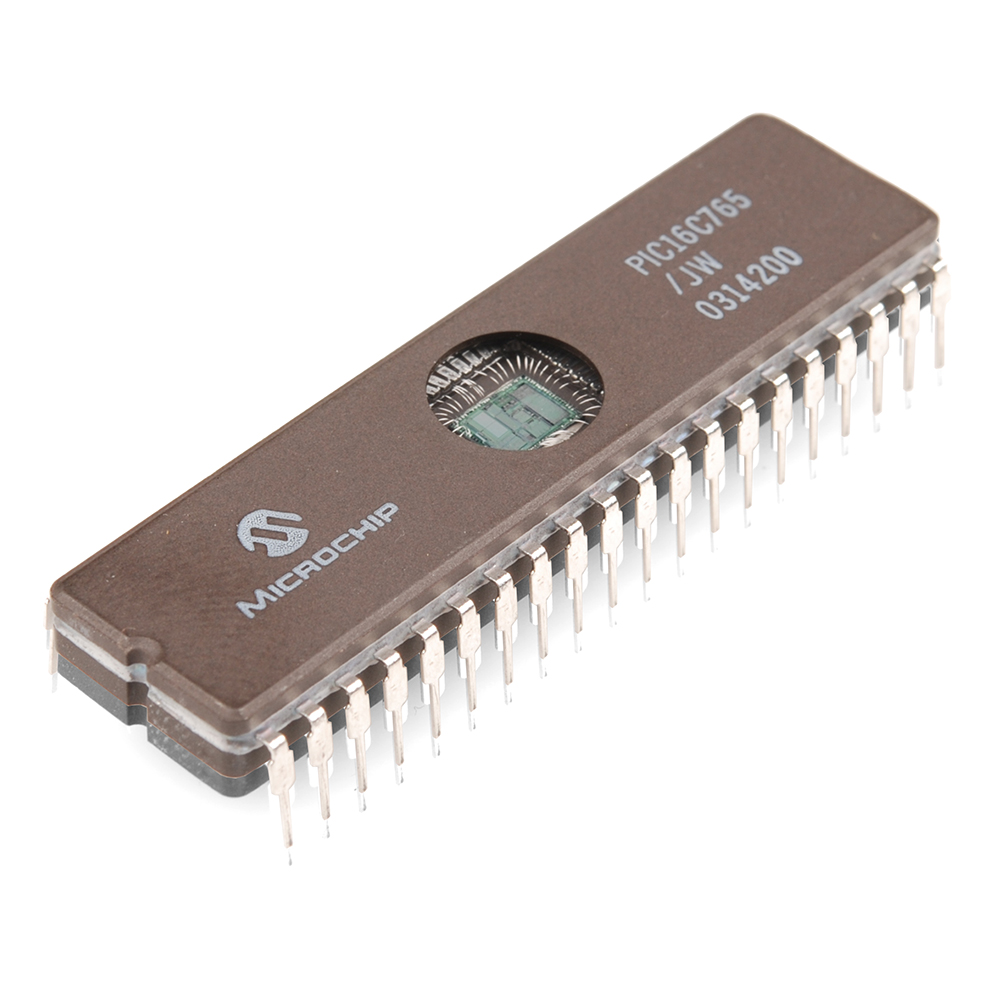
\includegraphics[height=5.2cm, trim=10 31 10 25, clip]{eprom-chip.jpg}% recorte del margen blanco (en bp; la foto mide 240 bp)
    \caption{Microcontrolador PIC16C765/JW: la versión ``JW'' tiene la memoria de programa en EPROM y se reconoce por la ventana.}
  \end{subfigure}\hfill
  \begin{subfigure}[b]{0.48\textwidth}
    \centering
    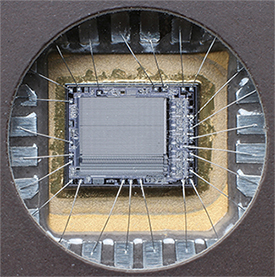
\includegraphics[height=5.2cm]{eprom-ventana.jpg}
    \caption{Detalle de la ventana de cuarzo: a través de ella se ve el chip de silicio y los hilos de conexión.}
  \end{subfigure}
  \caption{EPROM con ventana de cuarzo. Para borrarla se expone el chip a luz ultravioleta a través de la ventana; después se tapa con una etiqueta opaca para que la luz ambiente no la borre de a poco.}
\end{figure}

\subsection{EEPROM (\textit{Electrically Erasable PROM})}

Puede ser \textbf{borrada y reprogramada eléctricamente}, byte a byte, sin necesidad de extraer el chip del circuito. Permite actualizaciones en el propio sistema (\textit{In-System Programming}). Velocidad de escritura más lenta que la RAM; número de ciclos de escritura limitado (típicamente 100.000 a 1.000.000).

\subsection{Memoria Flash}

Es la evolución de la EEPROM. Comparte la capacidad de borrado y escritura eléctrica, pero opera por \textbf{bloques} en lugar de byte a byte, lo que la hace significativamente más rápida en operaciones de borrado. Combina:

\begin{itemize}
  \item Alta densidad de almacenamiento.
  \item No volatilidad.
  \item Lectura/escritura en el propio circuito.
  \item Velocidad de operación comparativamente alta.
  \item Bajo costo por bit.
\end{itemize}

Por estas razones es la tecnología dominante en memorias USB, tarjetas SD y en la \textbf{memoria de programa de los microcontroladores modernos} (incluyendo el ATmega328, que tiene 32 KB de Flash).

\textbf{Comparativa de tipos de ROM:}

\begin{table}[H]
\centering
\begin{tabular}{llll}
\toprule
Tipo & Programación & Borrado & Granularidad borrado \\
\midrule
ROM de máscara & En fábrica & No borrable & --- \\
PROM & Usuario, 1 vez & No borrable & --- \\
EPROM & Usuario & UV, total & Todo el chip \\
EEPROM & Eléctricamente & Eléctricamente & Byte a byte \\
Flash & Eléctricamente & Eléctricamente & Por bloques \\
\bottomrule
\end{tabular}
\end{table}

\section{Expansión de memoria}

En muchas aplicaciones la capacidad o el ancho de palabra de un único chip de memoria no son suficientes. Se pueden combinar varios chips para ampliar la memoria total del sistema. Existen dos técnicas:

\subsection{Expansión de palabra (ampliación de bits por posición)}

Se usa cuando el ancho de palabra de los chips es menor que el del bus de datos del sistema. Los chips se conectan \textbf{en paralelo}, compartiendo el mismo bus de direcciones y las mismas señales de control, pero cada uno aporta algunos bits del bus de datos.

\textbf{Ejemplo:} el bus de datos del sistema es de 8 bits, pero se tienen chips de 4 bits de ancho (organizados como 1K $\times$ 4). Se conectan dos chips en paralelo: uno proporciona D0--D3 y el otro D4--D7. Ambos chips responden a la misma dirección simultáneamente.

\tikzFigura{cap2/expansion-palabra}{Expansión de palabra: dos chips 1K$\times$4 en paralelo forman una memoria 1K$\times$8.}

$$\text{Chips necesarios} = \frac{\text{ancho de palabra del sistema}}{\text{ancho de palabra del chip}}$$

\subsection{Expansión de capacidad (ampliación de direcciones)}

Se usa cuando la cantidad de posiciones de un único chip es menor que la requerida. Los chips se conectan de forma que cada uno responde a un rango diferente de direcciones. Se usa la señal $\overline{CS}$ de cada chip para habilitarlo solo cuando el bus de direcciones está en su rango.

\textbf{Ejemplo:} se necesitan 4K posiciones de 8 bits, pero solo se tienen chips de 1K $\times$ 8. Se conectan 4 chips: el primero responde a las direcciones 0x000--0x3FF, el segundo a 0x400--0x7FF, y así sucesivamente. Un decodificador de 2 a 4 (por ejemplo, el 74139, o un 74138 usando 4 de sus 8 salidas) genera las señales $\overline{CS}$ individuales a partir de las líneas de mayor peso del bus de direcciones.

\tikzFigura{cap2/expansion-capacidad}{Expansión de capacidad: cuatro chips 1K$\times$8 y un decodificador 2 a 4 forman una memoria 4K$\times$8.}

$$\text{Chips necesarios} = \frac{\text{capacidad total requerida}}{\text{capacidad de cada chip}}$$

\subsection{Expansión combinada}

Es posible aplicar ambas técnicas simultáneamente para ampliar tanto el ancho de palabra como la cantidad de posiciones. En ese caso:

$$\text{Chips necesarios} = \frac{\text{capacidad total}}{\text{capacidad del chip}} \times \frac{\text{ancho de palabra del sistema}}{\text{ancho de palabra del chip}}$$

\chapter{Sistemas Microprogramables}

\section{Lógica cableada y lógica programada}

En electrónica digital se pueden diferenciar dos grandes enfoques para resolver un problema:

\textbf{Lógica cableada:} Para cada aplicación se diseña un circuito específico basado en compuertas lógicas. Una vez construido es muy difícil o imposible de modificar. El comportamiento del sistema queda determinado por el hardware.

\textbf{Lógica programada:} Un mismo dispositivo puede resolver distintos problemas simplemente cambiando su programa. El comportamiento del sistema queda determinado por el software que se le carga.

\section{Definición de sistema microprogramable}

Un sistema microprogramable es un dispositivo, o conjunto de dispositivos, de propósito general que se programa para resolver distintos problemas. Su versatilidad radica en que basta con cambiar el software para cambiar completamente su función.

Algunas aplicaciones típicas:

\begin{itemize}
  \item \textbf{Informática:} computadoras personales, periféricos (teclado, impresora, escáner).
  \item \textbf{Cálculo:} calculadoras científicas, supercomputadoras.
  \item \textbf{Procesos industriales:} PLCs para control de robots y líneas de montaje.
  \item \textbf{Electrodomésticos:} lavadoras, hornos, televisores, reproductores de audio/video.
  \item \textbf{Comunicaciones:} teléfonos fijos y móviles, equipos de red.
  \item \textbf{Automoción:} control de climatización, ABS, airbags.
  \item \textbf{Supervisión y alarmas:} ascensores, calefacción, alarmas contra incendio y robo.
  \item \textbf{Otros:} instrumentación, electromedicina, sistemas de navegación, tarjetas inteligentes (SUBE, monedero electrónico).
\end{itemize}

\section{Clasificación de los sistemas microprogramables}

Los sistemas microprogramables se clasifican según su grado de integración, capacidad de procesamiento y forma de trabajo:

\subsection{Microprocesadores}

El sistema está distribuido en varios circuitos integrados. El más importante es el \textbf{microprocesador}, que contiene únicamente la Unidad Central de Proceso (CPU). La memoria, los puertos de entrada/salida y demás periféricos son componentes externos que se interconectan mediante buses.

Se utiliza cuando se requieren grandes cantidades de memoria, alta velocidad o se prevén futuras ampliaciones. Ejemplo típico: la computadora personal.

\subsection{Microcontroladores}

Todo el sistema microprogramable ---CPU, memoria, puertos de E/S y periféricos--- está integrado en un \textbf{único circuito integrado}. Esto reduce el costo y el tamaño del sistema final, aunque su capacidad de procesamiento es menor que la de los microprocesadores. Son ideales para aplicaciones embebidas donde se necesita un procesador compacto y de bajo consumo.

Se encuentran en prácticamente todos los dispositivos electrónicos modernos: electrodomésticos, juguetes, instrumentos, automóviles, etc.

\subsection{Dispositivos PLDs}

Los PLD (\textit{Programmable Logic Device}) integran una matriz de compuertas lógicas cuya interconexión puede ser programada por el usuario. A diferencia de los microprocesadores y microcontroladores, \textbf{no están basados en una CPU} que lee instrucciones de una memoria: su lógica queda grabada en la estructura del dispositivo.

Son adecuados para resolver problemas combinacionales o secuenciales de alta velocidad pero de lógica fija, como decodificadores, máquinas de estado o interfaces de hardware.

\section{Hardware, Software y Firmware}

Un sistema microprogramable se compone de tres elementos:

\begin{itemize}
  \item \textbf{Hardware:} la parte física del sistema; el conjunto de circuitos electrónicos.
  \item \textbf{Software:} el conjunto de programas e instrucciones que se cargan en el sistema para indicarle qué hacer. También se denomina software al conjunto de lenguajes utilizados para escribir esos programas.
  \item \textbf{Firmware:} software grabado en la memoria interna del dispositivo que el usuario normalmente no puede modificar. Cumple la función de intermediario entre el hardware y el software de aplicación. En una PC, la BIOS es un ejemplo de firmware.
\end{itemize}

\section{Arquitectura de un sistema basado en CPU}

Todo sistema microprogramable ---ya sea basado en microprocesador o en microcontrolador--- comparte la misma estructura fundamental. Sus elementos esenciales son:

\begin{itemize}
  \item Reloj
  \item CPU (ALU + Registros + Unidad de Control)
  \item Memoria
  \item Unidad de Entrada/Salida
  \item Buses del sistema
\end{itemize}

\subsection{Reloj}

El reloj es un generador de señal cuadrada de frecuencia constante, normalmente producida por un cristal de cuarzo (aunque también pueden usarse osciladores RC). Todos los elementos del sistema operan sincronizados con esta señal, que determina la velocidad de trabajo del sistema.

A partir de la señal de reloj se define el \textbf{ciclo de máquina}, compuesto por dos fases:

\begin{enumerate}
  \item \textbf{Fase de búsqueda (Fetch):} la CPU lee la próxima instrucción de la memoria y la almacena en el registro correspondiente.
  \item \textbf{Fase de ejecución (Execute):} la CPU ejecuta la instrucción leída.
\end{enumerate}

Algunos microprocesadores completan una instrucción en un único ciclo de máquina; otros requieren varios ciclos para instrucciones más complejas. La frecuencia del reloj y la cantidad de ciclos por instrucción determinan juntos la velocidad real de procesamiento.

\subsection{CPU (Unidad Central de Proceso)}

Es el elemento más importante del sistema. Se encarga de:

\begin{itemize}
  \item Interpretar y ejecutar las instrucciones del programa.
  \item Generar las señales de control para coordinar el resto del sistema.
  \item Realizar las operaciones aritméticas y lógicas.
  \item Transferir datos hacia y desde la memoria.
\end{itemize}

La CPU está formada por tres bloques:

\subsubsection{Unidad Aritmético-Lógica (ALU)}

Es un circuito combinacional que realiza operaciones aritméticas (suma, resta, multiplicación) y lógicas (AND, OR, NOT, XOR), así como desplazamientos de bits. Las operaciones las realiza sobre datos provenientes de los registros internos o de posiciones de memoria, y deposita el resultado en un registro (habitualmente el acumulador).

\subsubsection{Registros}

Los registros son pequeñas memorias internas de alta velocidad donde la CPU almacena datos e instrucciones de manera temporal. Están formados por biestables y su tamaño (en bits) define la arquitectura del procesador (8, 16, 32 o 64 bits).

Los registros más importantes son:

\textbf{Registro acumulador:} almacena uno de los operandos de la ALU y recibe el resultado de la operación. Todas las operaciones aritméticas y lógicas pasan por él.

\textbf{Registro de estado (flags):} conjunto de biestables que reflejan el resultado de la última operación realizada por la ALU. Los flags más comunes son:

\begin{table}[H]
\centering
\begin{tabular}{lll}
\toprule
Flag & Nombre & Se activa cuando\ldots \\
\midrule
Z & Zero & El resultado de la operación es cero \\
C & Carry & Hubo acarreo en el bit de mayor peso \\
N / S & Negativo / Signo & El resultado es negativo \\
V / OV & Overflow & El resultado excede el rango del tipo de dato \\
I & Interrupt & Las interrupciones globales están habilitadas \\
\bottomrule
\end{tabular}
\end{table}

\textbf{Registros auxiliares o de propósito general:} registros que el programador puede usar libremente para almacenar datos intermedios. Su cantidad varía según la arquitectura.

\textbf{Stack Pointer (SP):} puntero que apunta a la cima de la pila (\textit{stack}). La pila es una zona de memoria con estructura LIFO (\textit{Last In, First Out}): el último dato en entrar es el primero en salir. Se utiliza para guardar la dirección de retorno cuando se llama a una subrutina, y para preservar el estado de los registros durante el manejo de interrupciones.

\textbf{Contador de Programa (PC):} registro que contiene la dirección de la próxima instrucción a ejecutar. Se incrementa automáticamente en cada ciclo de fetch. Cuando se produce un salto o llamada a subrutina, este registro se actualiza con la nueva dirección.

\subsubsection{Unidad de Control (UC)}

Gobierna el funcionamiento de todo el sistema. Recibe las instrucciones del programa, las decodifica mediante el \textbf{decodificador de instrucciones} y genera las señales de control necesarias para que cada elemento realice su tarea en el momento correcto. También contiene el Contador de Programa.

\subsection{Memoria}

La memoria almacena los programas y los datos que el sistema necesita para funcionar. Se divide en dos zonas funcionales:

\begin{itemize}
  \item \textbf{Memoria de programa:} contiene las instrucciones a ejecutar. No se modifica durante la ejecución. Suele implementarse en memoria no volátil (ROM, Flash).
  \item \textbf{Memoria de datos:} almacena los datos y resultados intermedios del programa. Se modifica constantemente durante la ejecución. Siempre es RAM (volátil).
\end{itemize}

\begin{notabox}
No confundir con las memorias de almacenamiento masivo (disco duro, pendrive), que son periféricos externos.
\end{notabox}

\subsection{Unidad de Entrada/Salida (E/S)}

Permite la comunicación del sistema con el mundo exterior. Está formada por registros que, controlados por los buses del sistema, permiten leer señales del exterior (entradas) o escribir señales hacia afuera (salidas). Su función principal es adaptar las velocidades y niveles lógicos del sistema interno con los de los dispositivos externos.

\subsection{Buses del sistema}

Los elementos del sistema se interconectan mediante \textbf{buses}: conjuntos de conductores paralelos que transportan información del mismo tipo. El número de líneas de un bus determina su \textbf{ancho} y por ende la cantidad de información que puede transmitirse simultáneamente.

En un sistema basado en CPU existen tres buses fundamentales:

\subsubsection{Bus de direcciones (\textit{Address Bus})}

Transporta la dirección de la posición de memoria o del registro de E/S que se desea acceder. Es \textbf{unidireccional}: solo la CPU pone datos en él.

La cantidad de líneas del bus de direcciones determina la cantidad máxima de posiciones de memoria que el sistema puede direccionar:

$$N_{\text{direcciones}} = 2^{N_{\text{líneas}}}$$

Por ejemplo, un bus de 16 líneas puede direccionar $2^{16} = 65.536$ posiciones. Si cada posición almacena 1 byte, la memoria máxima es 64 KB.

Las líneas se nombran A0 (bit de menor peso) a An (bit de mayor peso).

\subsubsection{Bus de datos (\textit{Data Bus})}

Transporta los datos entre la CPU, la memoria y los periféricos. Es \textbf{bidireccional}: los datos pueden ir en ambas direcciones según se trate de una lectura o escritura. Su ancho define la cantidad de bits que se transfieren en paralelo en cada operación.

Las líneas se nombran D0 a Dn.

\subsubsection{Bus de control (\textit{Control Bus})}

Transporta las señales de coordinación del sistema: órdenes de lectura/escritura, habilitación de dispositivos, señales de interrupción, reset, etc. Permite que todos los elementos del sistema funcionen en sincronía y sin conflictos en el uso de los buses compartidos.

\subsubsection{Operaciones de lectura y escritura}

\textbf{Escritura:} la CPU coloca la dirección en el bus de direcciones, activa la señal de escritura en el bus de control y coloca el dato en el bus de datos. El dispositivo seleccionado almacena el dato.

\textbf{Lectura:} la CPU coloca la dirección en el bus de direcciones y activa la señal de lectura en el bus de control. El dispositivo seleccionado deposita su contenido en el bus de datos, y la CPU lo lee. La operación de lectura es \textbf{no destructiva}: el dato sigue almacenado en la memoria después de ser leído.

\section{Arquitecturas Von Neumann y Harvard}

La relación entre la CPU y la memoria puede organizarse de dos maneras distintas:

\subsection{Arquitectura Von Neumann}

La CPU se conecta a una \textbf{única memoria} mediante un \textbf{único juego de buses}. Tanto las instrucciones del programa como los datos se almacenan en el mismo espacio de memoria y viajan por el mismo bus.

\imagenPendiente{diagrama de bloques Von Neumann (CPU --- bus único --- memoria única)}

\textbf{Limitaciones:}
\begin{itemize}
  \item El bus único genera un cuello de botella: mientras la CPU busca una instrucción no puede acceder a datos, y viceversa.
  \item El tamaño de las instrucciones está condicionado por el ancho del bus de datos.
\end{itemize}

Es la arquitectura típica de los microprocesadores de uso general (PCs).

\subsection{Arquitectura Harvard}

La CPU se conecta a \textbf{dos memorias separadas} mediante \textbf{dos juegos de buses independientes}: uno para instrucciones y otro para datos.

\imagenPendiente{diagrama de bloques Harvard (CPU --- bus de programa --- memoria de programa / bus de datos --- memoria de datos)}

\textbf{Ventajas:}
\begin{itemize}
  \item La CPU puede leer la próxima instrucción y acceder a datos \textbf{simultáneamente}, eliminando el cuello de botella.
  \item El ancho del bus de programa puede ser diferente al del bus de datos, permitiendo optimizar ambos de forma independiente.
  \item Aumenta significativamente la velocidad de procesamiento.
\end{itemize}

Es la arquitectura utilizada por la mayoría de los \textbf{microcontroladores}, incluyendo la familia AVR (ATmega).

\section{Software: instrucciones y lenguajes de programación}

\subsection{Formato de una instrucción}

Las instrucciones que ejecuta la CPU tienen dos partes:

\begin{lstlisting}[style=estilo-pseudocode]
+----------------------+----------------------+
|   Codigo de          |      Operando        |
|   operacion          |   (puede no estar)   |
+----------------------+----------------------+
\end{lstlisting}

\begin{itemize}
  \item \textbf{Código de operación:} indica qué hacer (sumar, restar, mover un dato, comparar, saltar\ldots).
  \item \textbf{Operando:} indica con qué dato realizar la operación, o la dirección de memoria donde se encuentra ese dato.
\end{itemize}

\subsection{Tipos de instrucciones}

\begin{itemize}
  \item \textbf{Aritméticas:} suma, resta, multiplicación, división.
  \item \textbf{Lógicas:} AND, OR, NOT, XOR.
  \item \textbf{Desplazamiento:} rotación y corrimiento de bits.
  \item \textbf{Transferencia de datos:} mover datos entre registros, entre registros y memoria, o entre registros y puertos E/S.
  \item \textbf{Salto:} condicionales (ejecutan un salto solo si se cumple una condición de los flags) e incondicionales (saltan siempre).
  \item \textbf{Control:} inicialización, detención, no-operación (NOP), habilitación/deshabilitación de interrupciones.
\end{itemize}

\subsection{Lenguajes de programación}

Para que un programador pueda escribir el programa, y para que luego ese programa pueda ser ejecutado por la CPU, existen distintos niveles de lenguaje:

\subsubsection{Lenguaje máquina (código máquina)}

Es el único lenguaje que la CPU entiende directamente: secuencias de bits (ceros y unos) que representan instrucciones y datos. Aunque es el más eficiente, es extremadamente difícil de escribir y leer por un ser humano.

\subsubsection{Lenguaje ensamblador (\textit{Assembler})}

Reemplaza los códigos binarios por \textbf{mnemónicos}: abreviaturas en inglés que recuerdan la función de cada instrucción (\texttt{MOV}, \texttt{ADD}, \texttt{JMP}, etc.). Las direcciones de memoria pueden referenciarse con etiquetas simbólicas. Es específico de cada arquitectura.

Un programa llamado \textbf{ensamblador} traduce el código escrito en lenguaje ensamblador al código máquina correspondiente.

\subsubsection{Lenguajes de alto nivel}

Son los más cercanos al lenguaje humano y los más fáciles de escribir y mantener. No están atados a una arquitectura específica, lo que permite reutilizar el código en distintos sistemas. Algunos ejemplos: C, C++, Python, Java, Basic.

Para ejecutarse, deben ser traducidos a código máquina mediante un \textbf{compilador} (que traduce todo el programa de una vez) o un \textbf{intérprete} (que traduce y ejecuta instrucción por instrucción).

En sistemas embebidos, el lenguaje más utilizado es \textbf{C}, por su combinación de legibilidad, eficiencia y acceso a bajo nivel de hardware.

\section{El ATmega328 en este curso}

El microcontrolador utilizado en este curso es el \textbf{ATmega328P}, fabricado por Microchip (familia AVR). Se trabaja sobre placas Arduino Nano como plataforma de desarrollo, pero \textbf{sin utilizar el framework ni las bibliotecas de Arduino}: se programa directamente en C, accediendo a los registros del hardware.

Características principales:

\begin{table}[H]
\centering
\begin{tabular}{ll}
\toprule
Característica & Valor \\
\midrule
Arquitectura & Harvard, RISC de 8 bits \\
Frecuencia máxima & 20 MHz \\
Memoria de programa & 32 KB Flash \\
Memoria de datos (RAM) & 2 KB SRAM \\
Memoria no volátil de datos & 1 KB EEPROM \\
Puertos de E/S digitales & Hasta 23 pines \\
Periféricos integrados & Timers, UART, SPI, I$^2$C, ADC (10 bits), Watchdog \\
\bottomrule
\end{tabular}
\end{table}

Al ser una arquitectura Harvard, el ATmega328 tiene buses separados para memoria de programa (Flash) y memoria de datos (SRAM), lo que le permite ejecutar la mayoría de las instrucciones en un solo ciclo de reloj.

En los bloques siguientes se verá en detalle cómo programar este microcontrolador: cómo se organizan sus registros internos, cómo se configuran sus puertos y cómo se utilizan sus periféricos.

\chapter{Pensamiento Computacional y Algoritmos}

\section{¿Qué es un algoritmo?}

Un \textbf{algoritmo} es una secuencia finita de pasos ordenados y precisos que describe cómo resolver un problema. Para que una secuencia de pasos sea considerada un algoritmo debe cumplir las siguientes características:

\begin{itemize}
    \item \textbf{Finito:} debe terminar en algún momento, no puede ejecutarse indefinidamente.
    \item \textbf{Preciso:} cada paso debe ser claro e inequívoco, sin ambigüedades.
    \item \textbf{Definido:} si se ejecuta dos veces con los mismos datos de entrada, siempre produce el mismo resultado.
    \item \textbf{Con entrada y salida:} puede recibir datos del exterior (entradas) y debe producir al menos un resultado (salida).
\end{itemize}

\begin{notabox}
Los algoritmos son independientes del lenguaje de programación. Se pueden expresar en lenguaje natural, en pseudocódigo o en un diagrama de flujo, y luego traducirse a cualquier lenguaje de programación.
\end{notabox}

\textbf{Ejemplo cotidiano --- receta de cocina:}
\begin{enumerate}
    \item Calentar agua hasta que hierva.
    \item Agregar los fideos.
    \item Esperar 8 minutos.
    \item Colar y servir.
\end{enumerate}

Este es un algoritmo: tiene pasos ordenados, es finito y produce un resultado determinado.

\section{Representación de algoritmos: el diagrama de flujo}

Un \textbf{diagrama de flujo} es una representación gráfica de un algoritmo. Utiliza símbolos estandarizados conectados por flechas que indican el orden de ejecución de los pasos.

\subsection{Símbolos básicos}

\tikzCircuito{cap4/simbolos-flujo}{Símbolos básicos del diagrama de flujo: forma de cada uno y para qué se usa.}

\subsection{Reglas generales}

\begin{itemize}
    \item Todo diagrama empieza con un símbolo \textbf{Inicio} y termina con uno o más símbolos \textbf{Fin}.
    \item Las flechas indican la dirección del flujo: normalmente de arriba hacia abajo y de izquierda a derecha.
    \item Un rombo de decisión siempre tiene exactamente \textbf{dos salidas}: una para cuando la condición es verdadera (Sí) y otra para cuando es falsa (No).
    \item No deben existir caminos que queden sin salida ni flechas que apunten ``al vacío''.
\end{itemize}

\section{Estructuras de control}

Todo algoritmo se construye combinando tres estructuras fundamentales:

\subsection{Secuencia}

Los pasos se ejecutan uno tras otro, en el orden en que aparecen. Es la estructura más simple.

\tikzCircuito{cap4/secuencia}{Estructura de secuencia: cálculo del área de un rectángulo.}

\textbf{Ejemplo:} calcular el área de un rectángulo.
\begin{enumerate}
    \item Leer base.
    \item Leer altura.
    \item Calcular área = base $\times$ altura.
    \item Mostrar área.
\end{enumerate}

\subsection{Decisión (selección)}

El flujo se divide en dos caminos según el resultado de una condición. Se evalúa una expresión lógica (verdadera o falsa) y se ejecuta uno u otro bloque de pasos.

\tikzCircuito{cap4/si-sino}{Estructura de decisión (si--sino): las ramas Sí y No se reúnen al final.}

\textbf{Ejemplo:} determinar si un número es positivo o negativo.

\begin{lstlisting}[style=estilo-pseudocode]
Si número > 0 entonces
    Mostrar "El número es positivo"
Sino
    Mostrar "El número es negativo o cero"
Fin Si
\end{lstlisting}

Las decisiones pueden encadenarse o anidarse para evaluar múltiples condiciones.

\subsection{Repetición (iteración)}

Un bloque de pasos se ejecuta más de una vez, mientras se cumpla una condición. Hay dos variantes principales:

\subsubsection{Repetir mientras (while --- condición al inicio)}

La condición se evalúa \textbf{antes} de ejecutar el bloque. Si la condición es falsa desde el principio, el bloque no se ejecuta nunca.

\tikzCircuito{cap4/mientras}{Estructura de repetición \emph{mientras}: la condición se evalúa antes del bloque.}

\begin{lstlisting}[style=estilo-pseudocode]
Mientras condición sea verdadera hacer
    [bloque de pasos]
Fin Mientras
\end{lstlisting}

\textbf{Ejemplo:} mostrar los números del 1 al 10.
\begin{lstlisting}[style=estilo-pseudocode]
contador = 1
Mientras contador <= 10 hacer
    Mostrar contador
    contador = contador + 1
Fin Mientras
\end{lstlisting}

\subsubsection{Repetir hasta (do-while --- condición al final)}

La condición se evalúa \textbf{después} de ejecutar el bloque, por lo que el bloque se ejecuta \textbf{al menos una vez}. En PSeInt, el bucle se repite \emph{mientras la condición sea falsa} y termina \emph{cuando la condición se vuelve verdadera}: se repite ``hasta que'' se cumpla.

\tikzCircuito{cap4/repetir-hasta}{Estructura de repetición \emph{repetir--hasta que}: primero se ejecuta el bloque y después se evalúa la condición.}

\begin{lstlisting}[style=estilo-pseudocode]
Repetir
    [bloque de pasos]
Hasta Que condición
\end{lstlisting}

\textbf{Ejemplo:} pedir un número hasta que sea positivo.
\begin{lstlisting}[style=estilo-pseudocode]
Repetir
    Leer numero
Hasta Que numero > 0
\end{lstlisting}

\begin{notabox}
\textbf{Mientras vs.\ repetir--hasta:} comparando los dos diagramas se ve la diferencia. En el \emph{mientras} el rombo está \textbf{antes} del bloque: si la condición es falsa de entrada, el bloque no se ejecuta nunca. En el \emph{repetir--hasta} el rombo está \textbf{después}: el bloque siempre se ejecuta al menos una vez. Además, el \emph{mientras} sigue repitiendo con \textbf{Sí}, y el \emph{repetir--hasta} sigue repitiendo con \textbf{No}.
\end{notabox}

\section{Variables}

Una \textbf{variable} es un espacio de memoria con nombre que almacena un valor que puede cambiar durante la ejecución del algoritmo.

Características:
\begin{itemize}
    \item Tiene un \textbf{nombre} (identificador) que la distingue de las demás.
    \item Almacena un \textbf{tipo de dato} (número entero, número decimal, texto, etc.).
    \item Su valor puede \textbf{leerse} (consultar qué tiene) o \textbf{escribirse} (asignarle un nuevo valor).
\end{itemize}

\subsection{Tipos de datos básicos}

\begin{table}[H]
\centering
\begin{tabular}{lp{5cm}l}
\toprule
Tipo & Descripción & Ejemplo \\
\midrule
Entero & Número sin decimales & 5, -3, 100 \\
Real & Número con decimales & 3.14, -0.5 \\
Carácter & Un símbolo de texto & 'A', '7' \\
Cadena & Texto (varios caracteres) & "Hola", "temperatura" \\
Lógico & Verdadero o falso & Verdadero, Falso \\
\bottomrule
\end{tabular}
\end{table}

\subsection{Asignación}

La asignación guarda un valor en una variable. En pseudocódigo se escribe con la flecha $\leftarrow$:

\begin{lstlisting}[style=estilo-pseudocode]
temperatura <- 25
resultado <- base * altura
nombre <- "Juan"
\end{lstlisting}

\section{Operadores}

\subsection{Aritméticos}

\begin{table}[H]
\centering
\begin{tabular}{cl}
\toprule
Operador & Operación \\
\midrule
\texttt{+} & Suma \\
\texttt{-} & Resta \\
\texttt{*} & Multiplicación \\
\texttt{/} & División \\
\texttt{MOD} & Módulo (resto de la división entera) \\
\bottomrule
\end{tabular}
\end{table}

\subsection{Relacionales (comparación)}

\begin{table}[H]
\centering
\begin{tabular}{cl}
\toprule
Operador & Significado \\
\midrule
\texttt{>} & Mayor que \\
\texttt{<} & Menor que \\
\texttt{>=} & Mayor o igual que \\
\texttt{<=} & Menor o igual que \\
\texttt{=} & Igual \\
\texttt{<>} & Distinto \\
\bottomrule
\end{tabular}
\end{table}

\subsection{Lógicos}

\begin{table}[H]
\centering
\begin{tabular}{cp{9cm}}
\toprule
Operador & Significado \\
\midrule
\texttt{Y} / \texttt{AND} & Verdadero solo si ambas condiciones son verdaderas \\
\texttt{O} / \texttt{OR} & Verdadero si al menos una condición es verdadera \\
\texttt{NO} / \texttt{NOT} & Invierte el valor lógico \\
\bottomrule
\end{tabular}
\end{table}

\section{Herramienta: PSeInt}

\textbf{PSeInt} es un programa que permite escribir y ejecutar algoritmos en pseudocódigo, y visualizarlos como diagrama de flujo de forma automática.

\subsection{Configuración del perfil}

Para este curso se usa el perfil \textbf{EEST1 VL}, disponible en el aula virtual (Moodle). Para cargarlo:

\begin{enumerate}
    \item Ir a \textbf{Configurar $\rightarrow$ Opciones del lenguaje (perfiles) $\rightarrow$ Cargar}.
    \item Seleccionar el archivo \texttt{EEST1\_VL}.
    \item Hacer clic en \textbf{Aceptar}.
\end{enumerate}

\subsection{Editar el diagrama de flujo}

Existen tres formas de acceder al modo de diagrama de flujo:

\begin{itemize}
    \item Hacer clic en el ícono de diagrama de flujo en la barra de menú.
    \item Ir a \textbf{Archivo $\rightarrow$ Editar diagrama de flujo}.
    \item Presionar \textbf{F7}.
\end{itemize}

\subsection{Ejecutar el algoritmo}

\begin{itemize}
    \item \textbf{Ejecución completa:} botón \textit{Ejecutar} (flecha verde), o \textbf{F9}.
    \item \textbf{Ejecución paso a paso:} botón \textit{Paso a paso} (ícono de pies), útil para seguir el flujo y detectar errores.
\end{itemize}

\section{Ejercicios}

Los siguientes ejercicios deben resolverse primero dibujando el diagrama de flujo en PSeInt y verificando su funcionamiento con distintos valores de entrada.

\subsection{Ejercicio 1 --- Suma de dos valores}

Realizar un algoritmo capaz de sumar 2 valores e informar el resultado.

\subsection{Ejercicio 2 --- Operación con tres valores}

Realizar un algoritmo que permita ingresar 3 valores, sumar los primeros 2, restarle el tercero al resultado, e informar el resultado final.

\textbf{Relación esperada:} resultado = (A + B) $-$ C

\subsection{Ejercicio 3 --- Módulo de un valor}

Realizar un algoritmo capaz de calcular el módulo (valor absoluto) de un número e informar el resultado. Recordar que el módulo devuelve el valor positivo: si el número es positivo lo devuelve igual, si es negativo lo invierte.

\begin{advertenciabox}
Este ejercicio introduce la estructura de decisión: se necesita evaluar si el número es negativo para invertirlo.
\end{advertenciabox}

\subsection{Ejercicio 4 --- Sensor de temperatura}

Realizar un algoritmo capaz de informar si hace calor o frío. Se ingresa un valor de temperatura y el algoritmo debe:

\begin{itemize}
    \item Si la temperatura supera los 26°C: informar ``hace calor''.
    \item Si la temperatura es menor a 22°C: informar ``hace frío''.
    \item En cualquier otro caso (entre 22° y 26°): no informar nada (temperatura agradable).
\end{itemize}

\begin{advertenciabox}
Este ejercicio introduce decisiones múltiples: más de una condición debe evaluarse.
\end{advertenciabox}

\subsection{Ejercicio 5 --- Promedio de una serie de valores}

Realizar un algoritmo capaz de calcular el promedio de todos los números ingresados. El ingreso termina cuando el usuario introduce un 0.

\begin{advertenciabox}
Este ejercicio introduce la estructura de repetición. El algoritmo no sabe de antemano cuántos números se van a ingresar: debe seguir pidiendo valores hasta que se ingrese un 0, y recién entonces calcular y mostrar el promedio.
\end{advertenciabox}

\textbf{Consideraciones:}
\begin{itemize}
    \item Llevar la cuenta de cuántos valores se ingresaron (contador).
    \item Llevar la suma acumulada de los valores.
    \item No incluir el 0 en el cálculo del promedio.
    \item Tener en cuenta el caso en que se ingrese 0 como primer valor (no hay valores para promediar).
\end{itemize}

\chapter{Introducción al Lenguaje C}

\section{Del diagrama de flujo al código}

En el bloque anterior aprendimos a representar algoritmos con diagramas de flujo. Ahora vamos a traducir esos diagramas a un lenguaje que la computadora puede compilar y ejecutar: el \textbf{lenguaje C}.

C es un lenguaje de propósito general creado en los años 70. Es el lenguaje más usado en sistemas embebidos y microcontroladores por dos razones principales: es \textbf{eficiente} (genera código compacto y rápido) y ofrece \textbf{acceso directo al hardware} (registros, puertos, memoria). Todo lo que aprendamos en este bloque se va a aplicar directamente en la programación del microcontrolador.

\section{Estructura de un programa en C}

Todo programa en C tiene la siguiente estructura mínima:

\begin{lstlisting}[style=estilo-c]
#include <stdio.h>      // Incluir biblioteca estándar de entrada/salida

int main(void) {        // Función principal — el programa empieza aquí
    // instrucciones
    return 0;           // Indicar que el programa terminó correctamente
}
\end{lstlisting}

\textbf{Elementos obligatorios:}

\begin{itemize}
    \item \texttt{\#include <stdio.h>}: incluye la biblioteca que permite usar \texttt{printf} y \texttt{scanf} (entrada y salida por consola). En programas para microcontrolador esto cambiará, pero por ahora la usamos para probar en la PC.
    \item \texttt{int main(void)}: función principal. Todo programa en C debe tener exactamente una función \texttt{main}. La ejecución empieza en la primera línea de \texttt{main} y termina cuando se llega al \texttt{return}.
    \item \texttt{\{ \}}: las llaves definen un \textbf{bloque} de código. Todo lo que está entre \texttt{\{} y \texttt{\}} pertenece a ese bloque.
    \item \texttt{;}: cada instrucción termina con punto y coma. Olvidarlo es uno de los errores más frecuentes.
    \item \texttt{// comentario}: el compilador ignora todo lo que está a la derecha de \texttt{//} en esa línea. Los comentarios sirven para explicar el código.
\end{itemize}

\section{Variables y tipos de datos}

Antes de usar una variable en C hay que \textbf{declararla}: indicar su nombre y el tipo de dato que va a almacenar.

\begin{lstlisting}[style=estilo-c]
tipo nombre;
tipo nombre = valor_inicial;
\end{lstlisting}

\subsection{Tipos de datos básicos}

\begin{table}[H]
\centering
\begin{tabularx}{\textwidth}{ll>{\raggedright\arraybackslash}X>{\raggedright\arraybackslash}X}
\toprule
Tipo & Tamaño típico & Rango aproximado & Uso \\
\midrule
\texttt{int} & 2 o 4 bytes & $-32.768$ a $32.767$ (2 bytes) & Números enteros \\
\texttt{unsigned int} & 2 o 4 bytes & 0 a 65.535 (2 bytes) & Enteros sin signo \\
\texttt{float} & 4 bytes & $\pm 3{,}4 \times 10^{38}$ & Números decimales (simple precisión) \\
\texttt{double} & 8 bytes & $\pm 1{,}7 \times 10^{308}$ & Números decimales (doble precisión) \\
\texttt{char} & 1 byte & $-128$ a $127$ & Un carácter ASCII o un entero de 8 bits \\
\texttt{unsigned char} & 1 byte & 0 a 255 & Byte sin signo --- muy usado en embebidos \\
\bottomrule
\end{tabularx}
\end{table}

\begin{notabox}
En programación de microcontroladores AVR, el tipo más usado es \texttt{uint8\_t} (equivalente a \texttt{unsigned char}, siempre 8 bits). Por ahora trabajamos con \texttt{int} y \texttt{float} para mayor comodidad.
\end{notabox}

\subsection{Ejemplos de declaración}

\begin{lstlisting}[style=estilo-c]
int edad;               // declara una variable entera sin valor inicial
int contador = 0;       // declara e inicializa en 0
float temperatura = 25.5;
char letra = 'A';
unsigned int suma = 0;
\end{lstlisting}

\subsection{Reglas para nombrar variables}

\begin{itemize}
    \item Solo letras, números y guion bajo \texttt{\_}. No puede empezar con un número.
    \item C distingue mayúsculas de minúsculas: \texttt{Temperatura} y \texttt{temperatura} son variables distintas.
    \item No se pueden usar palabras reservadas del lenguaje (\texttt{int}, \texttt{if}, \texttt{while}, \texttt{return}, etc.).
    \item Elegir nombres descriptivos: \texttt{temperatura} es mejor que \texttt{t} o \texttt{x}.
\end{itemize}

\section{Operadores}

\subsection{Aritméticos}

\begin{table}[H]
\centering
\begin{tabular}{cccc}
\toprule
Operador & Operación & Ejemplo & Resultado \\
\midrule
\texttt{+} & Suma & \texttt{3 + 2} & \texttt{5} \\
\texttt{-} & Resta & \texttt{5 - 3} & \texttt{2} \\
\texttt{*} & Multiplicación & \texttt{4 * 3} & \texttt{12} \\
\texttt{/} & División & \texttt{7 / 2} & \texttt{3} (entera si ambos son \texttt{int}) \\
\texttt{\%} & Módulo (resto) & \texttt{7 \% 2} & \texttt{1} \\
\bottomrule
\end{tabular}
\end{table}

\begin{advertenciabox}
\textbf{Atención con la división entera:} en C, dividir dos \texttt{int} descarta los decimales. \texttt{7 / 2} da \texttt{3}, no \texttt{3.5}. Para obtener el decimal hay que usar \texttt{float}: \texttt{7.0 / 2} da \texttt{3.5}.
\end{advertenciabox}

\subsection{Relacionales}

\begin{table}[H]
\centering
\begin{tabular}{cl}
\toprule
Operador & Significado \\
\midrule
\texttt{==} & Igual (doble signo --- no confundir con \texttt{=} de asignación) \\
\texttt{!=} & Distinto \\
\texttt{>} & Mayor que \\
\texttt{<} & Menor que \\
\texttt{>=} & Mayor o igual \\
\texttt{<=} & Menor o igual \\
\bottomrule
\end{tabular}
\end{table}

\subsection{Lógicos}

\begin{table}[H]
\centering
\begin{tabular}{cl}
\toprule
Operador & Significado \\
\midrule
\texttt{\&\&} & AND lógico \\
\texttt{||} & OR lógico \\
\texttt{!} & NOT lógico \\
\bottomrule
\end{tabular}
\end{table}

\subsection{Asignación}

\begin{lstlisting}[style=estilo-c]
x = 5;          // asigna 5 a x
x = x + 1;      // incrementa x en 1
x += 1;         // equivalente al anterior (forma abreviada)
x++;            // también equivalente — incremento en 1
x--;            // decremento en 1
\end{lstlisting}

\section{Entrada y salida por consola}

Para los ejercicios en PC usamos dos funciones de \texttt{<stdio.h>}:

\subsection{\texttt{printf} --- mostrar datos en pantalla}

\begin{lstlisting}[style=estilo-c]
printf("Hola mundo\n");             // imprime texto
printf("El resultado es %d\n", x); // imprime texto + valor de x (entero)
printf("Temperatura: %.2f\n", t);  // imprime t con 2 decimales
\end{lstlisting}

Los especificadores de formato más comunes:

\begin{table}[H]
\centering
\begin{tabular}{cl}
\toprule
Especificador & Tipo \\
\midrule
\texttt{\%d} & Entero (\texttt{int}) \\
\texttt{\%f} & Decimal (\texttt{float} o \texttt{double}) \\
\texttt{\%.2f} & Decimal con 2 cifras decimales \\
\texttt{\%c} & Carácter (\texttt{char}) \\
\texttt{\%s} & Cadena de texto \\
\bottomrule
\end{tabular}
\end{table}

El \texttt{\textbackslash n} al final provoca un salto de línea.

\subsection{\texttt{scanf} --- leer datos del teclado}

\begin{lstlisting}[style=estilo-c]
int x;
scanf("%d", &x);    // lee un entero y lo guarda en x

float t;
scanf("%f", &t);    // lee un decimal y lo guarda en t
\end{lstlisting}

\begin{notabox}
El \texttt{\&} antes del nombre de la variable es obligatorio en \texttt{scanf}. Indica la \textbf{dirección de memoria} donde se debe guardar el dato. Olvidarlo causa comportamiento impredecible.
\end{notabox}

\section{Estructuras de control}

\subsection{Secuencia}

Las instrucciones se ejecutan en orden, de arriba a abajo. No requiere ninguna sintaxis especial.

\begin{lstlisting}[style=estilo-c]
int a, b, resultado;
scanf("%d", &a);
scanf("%d", &b);
resultado = a + b;
printf("Resultado: %d\n", resultado);
\end{lstlisting}

\subsection{Decisión: \texttt{if} / \texttt{else}}

\begin{lstlisting}[style=estilo-c]
if (condición) {
    // se ejecuta si la condición es verdadera
} else {
    // se ejecuta si la condición es falsa (opcional)
}
\end{lstlisting}

Para condiciones encadenadas:

\begin{lstlisting}[style=estilo-c]
if (temperatura > 26) {
    printf("Hace calor\n");
} else if (temperatura < 22) {
    printf("Hace frio\n");
} else {
    printf("Temperatura agradable\n");
}
\end{lstlisting}

\begin{advertenciabox}
\textbf{Errores frecuentes:}
\begin{itemize}
    \item Usar \texttt{=} en lugar de \texttt{==} dentro del \texttt{if}: \texttt{if (x = 5)} asigna 5 a x y siempre es verdadero. Lo correcto es \texttt{if (x == 5)}.
    \item Olvidar las llaves \texttt{\{\}} cuando el bloque tiene más de una instrucción.
\end{itemize}
\end{advertenciabox}

\subsection{Repetición: \texttt{while}}

La condición se evalúa \textbf{antes} de cada iteración. Si es falsa desde el principio, el cuerpo no se ejecuta.

\begin{lstlisting}[style=estilo-c]
while (condición) {
    // cuerpo del bucle
}
\end{lstlisting}

\begin{lstlisting}[style=estilo-c]
int contador = 1;
while (contador <= 10) {
    printf("%d\n", contador);
    contador++;
}
\end{lstlisting}

\subsection{Repetición: \texttt{do-while}}

El cuerpo se ejecuta \textbf{al menos una vez}; la condición se evalúa al final.

\begin{lstlisting}[style=estilo-c]
do {
    // cuerpo del bucle
} while (condición);
\end{lstlisting}

\begin{lstlisting}[style=estilo-c]
int valor;
do {
    printf("Ingrese un numero positivo: ");
    scanf("%d", &valor);
} while (valor <= 0);
\end{lstlisting}

\subsection{Repetición: \texttt{for}}

Forma compacta de escribir un bucle cuando se conoce de antemano la cantidad de iteraciones.

\begin{lstlisting}[style=estilo-c]
for (inicialización; condición; actualización) {
    // cuerpo del bucle
}
\end{lstlisting}

\begin{lstlisting}[style=estilo-c]
for (int i = 1; i <= 10; i++) {
    printf("%d\n", i);
}
\end{lstlisting}

Equivale exactamente a:

\begin{lstlisting}[style=estilo-c]
int i = 1;
while (i <= 10) {
    printf("%d\n", i);
    i++;
}
\end{lstlisting}

\section{Equivalencia entre pseudocódigo y C}

\begin{table}[H]
\centering
\begin{tabular}{ll}
\toprule
Pseudocódigo (PSeInt) & C \\
\midrule
\texttt{Leer variable} & \texttt{scanf("\%d", \&variable);} \\
\texttt{Escribir "texto"} & \texttt{printf("texto\textbackslash n");} \\
\texttt{Escribir variable} & \texttt{printf("\%d\textbackslash n", variable);} \\
\texttt{variable \textleftarrow\ valor} & \texttt{variable = valor;} \\
\texttt{Si condición Entonces ... Fin Si} & \texttt{if (condición) \{ ... \}} \\
\texttt{Si ... Sino ... Fin Si} & \texttt{if (...) \{ ... \} else \{ ... \}} \\
\texttt{Mientras condición Hacer ... Fin Mientras} & \texttt{while (condición) \{ ... \}} \\
\texttt{Repetir ... Hasta Que condición} & \texttt{do \{ ... \} while (condición);} \\
\texttt{MOD} & \texttt{\%} \\
\texttt{Y} & \texttt{\&\&} \\
\texttt{O} & \texttt{||} \\
\texttt{NO} & \texttt{!} \\
\bottomrule
\end{tabular}
\end{table}

\section{Ejercicios: los algoritmos del TP en C}

Los siguientes programas son la traducción directa de los diagramas de flujo del Bloque 4. Se pueden compilar y ejecutar en cualquier compilador de C estándar (online: repl.it, OnlineGDB, Tutorialspoint; local: VSCode con GCC).

\subsection{Ejercicio 1 --- Suma de dos valores}

\begin{lstlisting}[style=estilo-c]
#include <stdio.h>

int main(void) {
    int a, b, resultado;

    printf("Ingrese el primer numero: ");
    scanf("%d", &a);

    printf("Ingrese el segundo numero: ");
    scanf("%d", &b);

    resultado = a + b;

    printf("La suma es: %d\n", resultado);

    return 0;
}
\end{lstlisting}

\subsection{Ejercicio 2 --- Operación con tres valores}

\begin{lstlisting}[style=estilo-c]
#include <stdio.h>

int main(void) {
    int a, b, c, resultado;

    printf("Ingrese el primer numero: ");
    scanf("%d", &a);

    printf("Ingrese el segundo numero: ");
    scanf("%d", &b);

    printf("Ingrese el tercer numero: ");
    scanf("%d", &c);

    resultado = (a + b) - c;

    printf("El resultado es: %d\n", resultado);

    return 0;
}
\end{lstlisting}

\subsection{Ejercicio 3 --- Módulo (valor absoluto)}

\begin{lstlisting}[style=estilo-c]
#include <stdio.h>

int main(void) {
    int numero, modulo;

    printf("Ingrese un numero: ");
    scanf("%d", &numero);

    if (numero < 0) {
        modulo = -numero;
    } else {
        modulo = numero;
    }

    printf("El modulo es: %d\n", modulo);

    return 0;
}
\end{lstlisting}

\begin{notabox}
La biblioteca estándar \texttt{<math.h>} tiene la función \texttt{abs()} que hace esto automáticamente, pero aquí lo implementamos manualmente para practicar la estructura \texttt{if/else}.
\end{notabox}

\subsection{Ejercicio 4 --- Sensor de temperatura}

\begin{lstlisting}[style=estilo-c]
#include <stdio.h>

int main(void) {
    float temperatura;

    printf("Ingrese la temperatura: ");
    scanf("%f", &temperatura);

    if (temperatura > 26.0) {
        printf("Hace calor\n");
    } else if (temperatura < 22.0) {
        printf("Hace frio\n");
    }

    return 0;
}
\end{lstlisting}

\begin{notabox}
Cuando la temperatura está entre 22° y 26° el programa no imprime nada, tal como pide el enunciado.
\end{notabox}

\subsection{Ejercicio 5 --- Promedio de una serie de valores}

\begin{lstlisting}[style=estilo-c]
#include <stdio.h>

int main(void) {
    int numero;
    float suma = 0;
    int cantidad = 0;

    printf("Ingrese numeros (0 para terminar):\n");

    scanf("%d", &numero);

    while (numero != 0) {
        suma = suma + numero;
        cantidad++;
        scanf("%d", &numero);
    }

    if (cantidad > 0) {
        printf("El promedio es: %.2f\n", suma / cantidad);
    } else {
        printf("No se ingresaron numeros.\n");
    }

    return 0;
}
\end{lstlisting}

\begin{notabox}
\textbf{Puntos importantes de este ejercicio:}
\begin{itemize}
    \item La suma se declara como \texttt{float} para que la división no pierda los decimales.
    \item El \texttt{if (cantidad > 0)} evita la división por cero si el usuario ingresa 0 inmediatamente.
    \item El 0 final \textbf{no se suma} porque la condición del \texttt{while} se evalúa antes de acumular.
\end{itemize}
\end{notabox}

\section{Entorno de desarrollo}

Para compilar y ejecutar programas en C se puede usar cualquiera de los siguientes entornos:

\textbf{Online (sin instalación):}
\begin{itemize}
    \item \texttt{replit.com} --- crea un proyecto de tipo C.
    \item \texttt{onlinegdb.com} --- compilador + depurador online.
    \item \texttt{tutorialspoint.com/compile\_c\_online.php}
\end{itemize}

\textbf{Local:}
\begin{itemize}
    \item \textbf{VSCode} + extensión C/C++ + compilador GCC (a través de MinGW en Windows).
\end{itemize}

\chapter{Programación de Microcontroladores en C}

%──────────────────────────────────────────────────────────────────────────────
\section{C estándar vs.\ C embebido}

En el Bloque 5 aprendimos C para correr programas en una PC. Al programar un
microcontrolador, el lenguaje es el mismo pero el contexto cambia completamente:

\begin{table}[H]
\centering
\begin{tabularx}{\textwidth}{>{\raggedright\arraybackslash}p{3.3cm}
    >{\raggedright\arraybackslash}X >{\raggedright\arraybackslash}X}
\toprule
 & \textbf{C en PC} & \textbf{C en microcontrolador} \\
\midrule
Sistema operativo & Sí (Windows, Linux) & No hay \\
Entrada/salida & Teclado, pantalla (\texttt{printf}, \texttt{scanf}) & Pines físicos del chip \\
Memoria & Abundante (GB) & Escasa (KB) \\
Punto de entrada & \texttt{main()} retorna cuando termina & \texttt{main()} nunca debe retornar --- bucle infinito \\
Bibliotecas estándar & \texttt{<stdio.h>}, \texttt{<math.h>}, etc. & Reemplazadas por bibliotecas del fabricante \\
\bottomrule
\end{tabularx}
\end{table}

En lugar de \texttt{\#include <stdio.h>} usaremos las bibliotecas de AVR:

\begin{lstlisting}[style=estilo-c]
#include <avr/io.h>        // definiciones de registros y pines del ATmega
#include <util/delay.h>    // función _delay_ms() para retardos
#include <avr/interrupt.h> // manejo de interrupciones
\end{lstlisting}

\subsection{Estructura básica de un programa embebido}

\begin{lstlisting}[style=estilo-c]
#include <avr/io.h>
#include <util/delay.h>

int main(void) {

    // --- INICIALIZACIÓN (se ejecuta una sola vez al encender) ---
    // Configurar puertos, registros, periféricos...

    // --- BUCLE PRINCIPAL (se ejecuta para siempre) ---
    while (1) {
        // lógica de la aplicación
    }

    return 0; // nunca se llega aquí, pero el compilador lo requiere
}
\end{lstlisting}

Esta estructura de \textbf{inicialización + bucle infinito} es el patrón fundamental de
todo programa embebido. El microcontrolador no tiene un sistema operativo que lo
controle: es el programa quien toma el control total del hardware desde el primer
momento.

%──────────────────────────────────────────────────────────────────────────────
\section{Los puertos de E/S del ATmega328}

El ATmega328 tiene tres puertos de E/S digitales: \textbf{PORTB}, \textbf{PORTC} y
\textbf{PORTD}, cada uno con hasta 8 pines. Cada puerto se controla mediante tres
registros de 8 bits:

\begin{table}[H]
\centering
\begin{tabular}{lp{10cm}}
\toprule
\textbf{Registro} & \textbf{Función} \\
\midrule
\texttt{DDRx} & \textit{Data Direction Register} --- define si cada pin es
    \textbf{entrada (0)} o \textbf{salida (1)} \\
\texttt{PORTx} & Si el pin es \textbf{salida}: escribe el nivel lógico
    (0 = LOW, 1 = HIGH). Si el pin es \textbf{entrada}: activa (1) o desactiva (0)
    la resistencia de pull-up interna \\
\texttt{PINx} & \textit{Port Input Pins} --- permite \textbf{leer} el estado actual
    de los pines (solo lectura) \\
\bottomrule
\end{tabular}
\end{table}

Donde \texttt{x} es \texttt{B}, \texttt{C} o \texttt{D} según el puerto.

\tikzCircuito{cap6/nano-pinout}{Mapa de pines del Arduino Nano y su correspondencia con los puertos del ATmega328P (PB, PC, PD)}

\subsection{Correspondencia Arduino Nano --- ATmega328}

\begin{table}[H]
\centering
\begin{tabular}{ccc}
\toprule
\textbf{Pin Arduino} & \textbf{Puerto ATmega} & \textbf{Bit} \\
\midrule
D0  & PORTD & 0 \\
D1  & PORTD & 1 \\
D2  & PORTD & 2 \\
D3  & PORTD & 3 \\
D4  & PORTD & 4 \\
D5  & PORTD & 5 \\
D6  & PORTD & 6 \\
D7  & PORTD & 7 \\
D8  & PORTB & 0 \\
D9  & PORTB & 1 \\
D10 & PORTB & 2 \\
D11 & PORTB & 3 \\
D12 & PORTB & 4 \\
D13 & PORTB & 5 \\
A0  & PORTC & 0 \\
A1  & PORTC & 1 \\
A2  & PORTC & 2 \\
A3  & PORTC & 3 \\
A4  & PORTC & 4 \\
A5  & PORTC & 5 \\
\bottomrule
\end{tabular}
\end{table}

%──────────────────────────────────────────────────────────────────────────────
\section{Operadores de manejo de bits}

Para configurar y controlar los registros del microcontrolador necesitamos
modificar bits individuales sin afectar los demás. Para eso usamos los
\textbf{operadores bitwise} (a nivel de bits):

\begin{table}[H]
\centering
\begin{tabularx}{\textwidth}{cl>{\raggedright\arraybackslash}X}
\toprule
\textbf{Operador} & \textbf{Nombre} & \textbf{Operación} \\
\midrule
\texttt{\&}  & AND bit a bit                    & El bit resultado es 1 solo si ambos operandos tienen 1 \\
\texttt{|}   & OR bit a bit                     & El bit resultado es 1 si al menos uno de los operandos tiene 1 \\
\texttt{\^{}}& XOR bit a bit                    & El bit resultado es 1 si los operandos son distintos \\
\texttt{\~{}}& NOT bit a bit                    & Invierte todos los bits \\
\texttt{<<}  & Desplazamiento a la izquierda    & Desplaza los bits hacia la izquierda N posiciones \\
\texttt{>>}  & Desplazamiento a la derecha      & Desplaza los bits hacia la derecha N posiciones \\
\bottomrule
\end{tabularx}
\end{table}

\subsection{Desplazamiento de bits}

El operador \texttt{<<} es clave para crear \textbf{máscaras}: valores que tienen un
único bit en 1 en la posición deseada.

\begin{lstlisting}[style=estilo-c]
1 << 0  ->  0b00000001  ->  0x01   (bit 0)
1 << 1  ->  0b00000010  ->  0x02   (bit 1)
1 << 3  ->  0b00001000  ->  0x08   (bit 3)
1 << 7  ->  0b10000000  ->  0x80   (bit 7)
\end{lstlisting}

En la biblioteca \texttt{<avr/io.h>} los bits de cada registro ya tienen nombres
definidos. Por ejemplo, \texttt{PD3} es el bit 3 del puerto D, y su valor es
\texttt{3}. Entonces \texttt{(1 << PD3)} genera la máscara para ese bit.

%──────────────────────────────────────────────────────────────────────────────
\section{Técnicas de enmascarado}

\subsection{Poner un bit en 1 (SET)}

Se usa OR con una máscara que tiene 1 en la posición deseada:

\begin{lstlisting}[style=estilo-c]
PORTD = PORTD | (1 << PD3);   // pone el bit 3 de PORTD en 1
PORTD |= (1 << PD3);           // forma abreviada (equivalente)
\end{lstlisting}

Ejemplo: \texttt{PORTD = 0b00000000}, aplicar máscara \texttt{0b00001000}:

\begin{lstlisting}[style=estilo-c]
  0 0 0 0 0 0 0 0   (PORTD original)
| 0 0 0 0 1 0 0 0   (máscara: 1 << PD3)
= 0 0 0 0 1 0 0 0   (resultado: solo el bit 3 cambió)
\end{lstlisting}

\subsection{Poner un bit en 0 (CLEAR)}

Se usa AND con el complemento de la máscara (\texttt{\~{}}):

\begin{lstlisting}[style=estilo-c]
PORTD = PORTD & ~(1 << PD3);  // pone el bit 3 de PORTD en 0
PORTD &= ~(1 << PD3);          // forma abreviada
\end{lstlisting}

Ejemplo: \texttt{PORTD = 0b11111111}, aplicar máscara:

\begin{lstlisting}[style=estilo-c]
  1 1 1 1 1 1 1 1   (PORTD original)
& 1 1 1 1 0 1 1 1   (~(1 << PD3): todos 1 excepto el bit 3)
= 1 1 1 1 0 1 1 1   (resultado: solo el bit 3 se puso en 0)
\end{lstlisting}

\subsection{Invertir un bit (TOGGLE)}

Se usa XOR con la máscara:

\begin{lstlisting}[style=estilo-c]
PORTD ^= (1 << PD3);   // invierte el bit 3 de PORTD
\end{lstlisting}

\subsection{Leer el estado de un bit}

Se usa AND con la máscara y se compara con cero:

\begin{lstlisting}[style=estilo-c]
if (PIND & (1 << PD2)) {
    // el bit 2 de PIND está en 1 (pin en HIGH)
}

if (!(PIND & (1 << PD2))) {
    // el bit 2 de PIND está en 0 (pin en LOW)
}
\end{lstlisting}

%──────────────────────────────────────────────────────────────────────────────
\section{Configuración de puertos (TP1)}

\subsection{Configurar un pin como salida}

Para usar un pin como salida, se pone en 1 el bit correspondiente en \texttt{DDRx}:

\begin{lstlisting}[style=estilo-c]
DDRD |= (1 << PD5);    // PD5 (pin D5) como salida
\end{lstlisting}

\subsection{Configurar un pin como entrada}

Para usar un pin como entrada, se pone en 0 el bit correspondiente en \texttt{DDRx}:

\begin{lstlisting}[style=estilo-c]
DDRD &= ~(1 << PD2);   // PD2 (pin D2) como entrada
\end{lstlisting}

\subsection{Activar la resistencia de pull-up interna}

Cuando un pin es entrada, se puede activar su resistencia pull-up interna
poniéndolo en 1 en \texttt{PORTx}. Esto evita que el pin ``flote'' cuando no hay
nada conectado:

\begin{lstlisting}[style=estilo-c]
DDRD  &= ~(1 << PD2);  // PD2 como entrada
PORTD |=  (1 << PD2);  // activa pull-up interno en PD2
\end{lstlisting}

Con pull-up activo, la lógica se \textbf{invierte}: el pin lee 1 cuando el pulsador
está suelto y 0 cuando está presionado (porque el pulsador conecta el pin a GND).

\subsection{Escribir en un pin de salida}

\begin{lstlisting}[style=estilo-c]
PORTD |=  (1 << PD5);  // pone PD5 en HIGH (LED encendido)
PORTD &= ~(1 << PD5);  // pone PD5 en LOW  (LED apagado)
\end{lstlisting}

\subsection{Leer un pin de entrada}

\begin{lstlisting}[style=estilo-c]
if (!(PIND & (1 << PD2))) {
    // pulsador presionado (con pull-up: pulsador conecta a GND -> lee 0)
}
\end{lstlisting}

\subsection{Ejemplo completo --- TP1: un pulsador controla un LED}

\begin{lstlisting}[style=estilo-c]
#include <avr/io.h>

int main(void) {

    // Inicialización
    DDRD |=  (1 << PD5);   // PD5 (D5) como salida -> LED
    DDRD &= ~(1 << PD2);   // PD2 (D2) como entrada -> pulsador
    PORTD |= (1 << PD2);   // activar pull-up en PD2

    while (1) {
        if (!(PIND & (1 << PD2))) {
            // pulsador presionado -> encender LED
            PORTD |= (1 << PD5);
        } else {
            // pulsador suelto -> apagar LED
            PORTD &= ~(1 << PD5);
        }
    }

    return 0;
}
\end{lstlisting}

%──────────────────────────────────────────────────────────────────────────────
\section{Retardos}

La función \texttt{\_delay\_ms(n)} detiene la ejecución durante \texttt{n}
milisegundos. Es un retardo \textbf{bloqueante}: mientras espera, el programa no
hace nada más.

\begin{lstlisting}[style=estilo-c]
#include <util/delay.h>

_delay_ms(500);    // espera 500 ms
_delay_us(100);    // espera 100 microsegundos
\end{lstlisting}

\begin{importantebox}
Para que \texttt{\_delay\_ms} funcione correctamente, el compilador debe saber a qué
frecuencia corre el microcontrolador. Esto se configura con la constante \texttt{F\_CPU}
antes del include, o en las opciones del compilador:
\begin{lstlisting}[style=estilo-c]
#define F_CPU 16000000UL   // 16 MHz (Arduino Nano)
#include <util/delay.h>
\end{lstlisting}
\end{importantebox}

Los retardos son útiles para efectos simples (parpadeo, secuencias de LEDs), pero
tienen una desventaja importante: \textbf{bloquean todo el programa}. Mientras
espera, el microcontrolador no puede leer pulsadores, actualizar displays ni hacer
otra cosa. Para aplicaciones más complejas se usan los \textbf{timers con
interrupciones} (TP5).

%──────────────────────────────────────────────────────────────────────────────
\section{Escribir en el puerto completo}

Cuando se controlan varios pines simultáneamente (por ejemplo, 8 LEDs o los 7
segmentos de un display), conviene escribir en el registro completo en lugar de bit
a bit:

\begin{lstlisting}[style=estilo-c]
PORTD = 0b00110101;   // escribe el valor completo en el puerto D
PORTB = 0x3F;         // escribe 0x3F en el puerto B (en hexadecimal)
\end{lstlisting}

\begin{advertenciabox}
Esto sobreescribe \textbf{todos} los bits del puerto. Si algunos pines están
configurados como entradas (con pull-up), sobreescribir el registro afectará también
a esos bits. Hay que tener en cuenta qué pines se usan para qué.
\end{advertenciabox}

%──────────────────────────────────────────────────────────────────────────────
\section{Display de 7 segmentos (TP4)}

Un display de 7 segmentos tiene 7 LEDs (a, b, c, d, e, f, g) y opcionalmente un
punto decimal (dp), que se encienden en distintas combinaciones para mostrar un
dígito.

\tikzCircuito{cap6/display-7seg}{Disposición de los segmentos a--g en un display de 7 segmentos de cátodo común}

Existen dos tipos:
\begin{itemize}
    \item \textbf{Ánodo común:} el cátodo de cada segmento se conecta al pin del
          microcontrolador. Para encender un segmento se pone el pin en \textbf{LOW (0)}.
    \item \textbf{Cátodo común:} el ánodo de cada segmento se conecta al pin del
          microcontrolador. Para encender un segmento se pone el pin en \textbf{HIGH (1)}.
\end{itemize}

Si conectamos los segmentos a, b, c, d, e, f, g del display a los bits 0..6 del
\texttt{PORTD} (cátodo común), la tabla de patrones para mostrar los dígitos 0 al 9 es:

\begin{table}[H]
\centering
\begin{tabular}{ccccccccc}
\toprule
\textbf{Dígito} & \textbf{g} & \textbf{f} & \textbf{e} & \textbf{d} &
\textbf{c} & \textbf{b} & \textbf{a} & \textbf{Hex} \\
\midrule
0 & 0 & 1 & 1 & 1 & 1 & 1 & 1 & \texttt{0x3F} \\
1 & 0 & 0 & 0 & 0 & 1 & 1 & 0 & \texttt{0x06} \\
2 & 1 & 0 & 1 & 1 & 0 & 1 & 1 & \texttt{0x5B} \\
3 & 1 & 0 & 0 & 1 & 1 & 1 & 1 & \texttt{0x4F} \\
4 & 1 & 1 & 0 & 0 & 1 & 1 & 0 & \texttt{0x66} \\
5 & 1 & 1 & 0 & 1 & 1 & 0 & 1 & \texttt{0x6D} \\
6 & 1 & 1 & 1 & 1 & 1 & 0 & 1 & \texttt{0x7D} \\
7 & 0 & 0 & 0 & 0 & 1 & 1 & 1 & \texttt{0x07} \\
8 & 1 & 1 & 1 & 1 & 1 & 1 & 1 & \texttt{0x7F} \\
9 & 1 & 1 & 0 & 1 & 1 & 1 & 1 & \texttt{0x6F} \\
\bottomrule
\end{tabular}
\caption{Patrones de display 7 segmentos --- cátodo común, segmentos en \texttt{PORTD} bits 0..6}
\end{table}

En el código se almacena esta tabla en un arreglo y se indexa con el dígito a mostrar:

\begin{lstlisting}[style=estilo-c]
#include <avr/io.h>

// Patrones para dígitos 0-9 (cátodo común, segmentos en PORTD bits 0..6)
const uint8_t digitos[10] = {
    0x3F, // 0
    0x06, // 1
    0x5B, // 2
    0x4F, // 3
    0x66, // 4
    0x6D, // 5
    0x7D, // 6
    0x07, // 7
    0x7F, // 8
    0x6F  // 9
};

int main(void) {
    DDRD = 0x7F;          // PD0..PD6 como salidas (segmentos a-g)
    PORTD = digitos[0];   // mostrar el dígito 0

    while (1) {
        // la lógica de conteo iría aquí
    }
    return 0;
}
\end{lstlisting}

%──────────────────────────────────────────────────────────────────────────────
\section{Timers e interrupciones (TP5)}

\subsection{El problema del código bloqueante}

Con \texttt{\_delay\_ms()} el microcontrolador se queda ``dormido'' esperando. No
puede atender pulsadores ni actualizar displays mientras espera. Esto es el
\textbf{código bloqueante}.

La solución son los \textbf{timers con interrupciones}: el timer cuenta en segundo
plano y cuando llega a un valor configurado, interrumpe al programa principal para
ejecutar una función especial (ISR).

\subsection{Interrupciones}

Una \textbf{interrupción} es una señal que detiene temporalmente la ejecución del
programa principal para atender un evento (el timer llegó al valor, llegó un dato
por UART, cambió un pin, etc.). Al terminar la función de interrupción, el programa
principal continúa desde donde fue interrumpido.

Para usar interrupciones:

\begin{enumerate}
    \item Configurar la fuente de interrupción (timer, pin externo, etc.).
    \item Definir la función ISR (\textit{Interrupt Service Routine}) que se ejecutará.
    \item Habilitar las interrupciones globales con \texttt{sei()}.
\end{enumerate}

\begin{lstlisting}[style=estilo-c]
#include <avr/io.h>
#include <avr/interrupt.h>

// Función ISR: se ejecuta automáticamente cuando ocurre la interrupción
ISR(TIMER0_COMPA_vect) {
    // código que se ejecuta cada 1 ms (modo CTC, comparación con OCR0A)
}

int main(void) {
    // configurar el timer...

    sei();    // habilitar interrupciones globales

    while (1) {
        // programa principal — sin delays bloqueantes
    }
    return 0;
}
\end{lstlisting}

La función ISR \textbf{no se llama} desde el programa: la llama automáticamente el
hardware cuando ocurre el evento. El argumento de \texttt{ISR} es el \textbf{vector
de interrupción} que indica la fuente.

\subsection{Vectores de interrupción del ATmega328}

Los principales vectores disponibles son:

\begin{lstlisting}[style=estilo-c]
INT0_vect          // Interrupción externa en pin INT0 (D2)
INT1_vect          // Interrupción externa en pin INT1 (D3)
PCINT0_vect        // Cambio de pin en PORTB
PCINT1_vect        // Cambio de pin en PORTC
PCINT2_vect        // Cambio de pin en PORTD
TIMER0_OVF_vect    // Desbordamiento del Timer 0
TIMER0_COMPA_vect  // Comparación A del Timer 0
TIMER1_OVF_vect    // Desbordamiento del Timer 1
TIMER1_COMPA_vect  // Comparación A del Timer 1
TIMER2_OVF_vect    // Desbordamiento del Timer 2
USART_RX_vect      // Recepción UART completa
ADC_vect           // Conversión ADC completa
TWI_vect           // I²C (Two Wire Interface)
SPI_STC_vect       // SPI transferencia completa
\end{lstlisting}

\subsection{Configuración del Timer 0 en modo CTC}

El modo CTC (\textit{Clear Timer on Compare Match}) hace que el contador se reinicie
automáticamente a 0 cada vez que alcanza el valor cargado en el registro
\texttt{OCR0A}, generando la interrupción \texttt{TIMER0\_COMPA\_vect}. Esto permite
obtener intervalos de tiempo exactos y predecibles sin depender del período de
desbordamiento.

El valor de \texttt{OCR0A} se calcula con la fórmula:

$$\text{OCR0A} = \frac{F_{\text{CPU}}}{\text{prescaler} \times f_{\text{interrupción}}} - 1$$

Para obtener una interrupción cada \textbf{1 ms} (1000 Hz) con el ATmega a 16 MHz y
preescalador 64:

$$OCR0A = \frac{16.000.000}{64 \times 1000} - 1 = 250 - 1 = 249$$

\begin{lstlisting}[style=estilo-c]
// Configurar Timer 0 en modo CTC — interrupción cada 1 ms
// F_CPU = 16 MHz, preescalador = 64, OCR0A = 249
TCCR0A = (1 << WGM01);                 // modo CTC
TCCR0B = (1 << CS01) | (1 << CS00);   // preescalador 64
OCR0A  = 249;                          // comparación: interrupt cada 1 ms

// Habilitar interrupción por comparación A
TIMSK0 = (1 << OCIE0A);
\end{lstlisting}

En modo CTC el contador no desborda: sube de 0 a \texttt{OCR0A}, genera la
interrupción y vuelve a 0. El período de la interrupción es exactamente 1 ms, lo
que hace muy simple llevar cuentas de tiempo en la ISR (cada llamada = 1 ms).

\subsection{Ejemplo --- parpadeo de LED sin código bloqueante}

La ISR se ejecuta cada 1 ms. Contando 500 llamadas se obtiene un período de 500 ms
$\rightarrow$ el LED parpadea a 1 Hz (500 ms encendido, 500 ms apagado).

\begin{lstlisting}[style=estilo-c]
#define F_CPU 16000000UL
#include <avr/io.h>
#include <avr/interrupt.h>

volatile uint16_t contador_ms = 0;

ISR(TIMER0_COMPA_vect) {           // se ejecuta cada 1 ms
    contador_ms++;
    if (contador_ms >= 500) {      // 500 ms
        contador_ms = 0;
        PORTB ^= (1 << PB5);       // toggle LED (pin D13)
    }
}

int main(void) {
    DDRB |= (1 << PB5);            // D13 como salida

    // Timer 0 — modo CTC — 1 ms
    TCCR0A = (1 << WGM01);
    TCCR0B = (1 << CS01) | (1 << CS00);   // preescalador 64
    OCR0A  = 249;
    TIMSK0 = (1 << OCIE0A);

    sei();

    while (1) {
        // el programa principal puede hacer otras cosas sin bloqueos
    }
    return 0;
}
\end{lstlisting}

\begin{notabox}
\textbf{La palabra clave \texttt{volatile}:} cuando una variable se modifica dentro
de una ISR y se usa fuera de ella, \textbf{debe declararse \texttt{volatile}}. Esto
le indica al compilador que no optimice los accesos a esa variable, ya que puede
cambiar en cualquier momento por la interrupción.
\end{notabox}

%──────────────────────────────────────────────────────────────────────────────
\section{Multiplexado de displays (TP6)}

Cuando se usan varios displays de 7 segmentos, conectar cada uno con 7 pines propios
requeriría demasiados pines del microcontrolador. La solución es el
\textbf{multiplexado}: compartir los 7 pines de segmentos entre todos los displays y
activar un display a la vez, rotando muy rápido ($>$50 Hz) para que el ojo humano
perciba todos encendidos simultáneamente.

\tikzCircuito{cap6/mux-displays}{Esquema de multiplexado de 4 displays de 7 segmentos: segmentos compartidos, selección individual por dígito}

\subsection{Principio de funcionamiento}

\begin{enumerate}
    \item Activar display 1: encender su pin de selección (common), escribir el
          dígito 1 en los segmentos.
    \item Pequeña espera ($\sim$2 ms).
    \item Apagar display 1, activar display 2: escribir el dígito 2 en los segmentos.
    \item Pequeña espera ($\sim$2 ms).
    \item Repetir para displays 3 y 4.
    \item Volver al display 1.
\end{enumerate}

Si la rotación es más rápida que $\sim$20 ms por display (50 Hz), el parpadeo es
imperceptible.

\subsection{Implementación con Timer 0}

El multiplexado se implementa en la ISR del Timer 0, sin bloquear el programa
principal:

\begin{lstlisting}[style=estilo-c]
#define F_CPU 16000000UL
#include <avr/io.h>
#include <avr/interrupt.h>

// Patrones de dígitos (cátodo común)
const uint8_t digitos[10] = {
    0x3F, 0x06, 0x5B, 0x4F, 0x66,
    0x6D, 0x7D, 0x07, 0x7F, 0x6F
};

// Pines de selección de cada display (en PORTB)
#define SEL0  PB0
#define SEL1  PB1
#define SEL2  PB2
#define SEL3  PB3

volatile uint8_t display_actual = 0;
uint8_t valores[4] = {1, 2, 3, 4};  // dígitos a mostrar en cada display

// ISR cada 1 ms — rota entre los 4 displays
// Cada display se muestra 1 ms -> frecuencia de refresco = 1/(4x1ms) = 250 Hz
ISR(TIMER0_COMPA_vect) {
    // Apagar todos los displays
    PORTB &= ~((1<<SEL0)|(1<<SEL1)|(1<<SEL2)|(1<<SEL3));

    // Escribir el dígito del display actual en los segmentos
    PORTD = digitos[valores[display_actual]];

    // Activar solo el display actual
    PORTB |= (1 << (SEL0 + display_actual));

    // Avanzar al siguiente display
    display_actual++;
    if (display_actual >= 4) display_actual = 0;
}

int main(void) {
    DDRD = 0x7F;                    // PD0..PD6 como salidas (segmentos)
    DDRB |= (1<<SEL0)|(1<<SEL1)|(1<<SEL2)|(1<<SEL3);  // selección

    // Timer 0 — modo CTC — 1 ms
    TCCR0A = (1 << WGM01);
    TCCR0B = (1 << CS01) | (1 << CS00);   // preescalador 64
    OCR0A  = 249;
    TIMSK0 = (1 << OCIE0A);

    sei();

    while (1) {
        // el programa principal puede modificar valores[] en cualquier momento
    }
    return 0;
}
\end{lstlisting}

%──────────────────────────────────────────────────────────────────────────────
\section{Eliminación de rebote por software}

Los pulsadores mecánicos ``rebotan'' al presionarse: hacen contacto y lo rompen
varias veces en pocos milisegundos antes de estabilizarse. Esto puede interpretarse
como múltiples pulsaciones.

\subsection{Método bloqueante (simple, para aprender)}

Esperar un tiempo mayor que el rebote ($\sim$20 ms) después de detectar el primer
flanco:

\begin{lstlisting}[style=estilo-c]
if (!(PIND & (1 << PD2))) {         // detectar flanco de bajada
    _delay_ms(20);                   // esperar que termine el rebote
    if (!(PIND & (1 << PD2))) {     // verificar que sigue presionado
        // acción al presionar
    }
}
\end{lstlisting}

\subsection{Método por detección de flanco (no bloqueante, TP5)}

Se guarda el estado anterior del pin y se actúa solo cuando hay un \textbf{cambio de
estado} (de 1 a 0 = flanco de bajada, de 0 a 1 = flanco de subida). El conteo de
rebotes se hace en la ISR del timer:

\begin{lstlisting}[style=estilo-c]
volatile uint8_t estado_anterior = 1;   // con pull-up, inicial = 1 (suelto)
volatile uint8_t contador_rebote = 0;

// ISR cada 1 ms — muestreo del pulsador
ISR(TIMER0_COMPA_vect) {
    uint8_t estado_actual = (PIND >> PD2) & 1;

    if (estado_actual != estado_anterior) {
        contador_rebote++;
        if (contador_rebote >= 20) {     // 20 lecturas estables = 20 ms
            estado_anterior = estado_actual;
            contador_rebote = 0;
            if (estado_actual == 0) {
                // flanco de bajada confirmado -> pulsador presionado
            }
        }
    } else {
        contador_rebote = 0;
    }
}
\end{lstlisting}

%──────────────────────────────────────────────────────────────────────────────
\section{Resumen de registros del ATmega328 usados en los TPs}

\begin{table}[H]
\centering
\begin{tabular}{lp{9cm}}
\toprule
\textbf{Registro} & \textbf{Función} \\
\midrule
\texttt{DDRB}, \texttt{DDRC}, \texttt{DDRD} & Dirección de datos de cada puerto \\
\texttt{PORTB}, \texttt{PORTC}, \texttt{PORTD} & Escritura de salidas / pull-ups de entradas \\
\texttt{PINB}, \texttt{PINC}, \texttt{PIND} & Lectura del estado de los pines \\
\texttt{TCCR0A}, \texttt{TCCR0B} & Control del Timer 0 (modo y preescalador) \\
\texttt{TCCR1A}, \texttt{TCCR1B} & Control del Timer 1 \\
\texttt{TIMSK0} & Habilitación de interrupciones del Timer 0 \\
\texttt{TIMSK1} & Habilitación de interrupciones del Timer 1 \\
\texttt{TCNT0} & Valor actual del contador del Timer 0 \\
\texttt{OCR0A}, \texttt{OCR0B} & Registros de comparación del Timer 0 \\
\texttt{SREG} & Registro de estado (flags de la CPU, incluye el bit I de interrupciones globales) \\
\bottomrule
\end{tabular}
\caption{Registros del ATmega328 utilizados en los TPs}
\end{table}

\begin{notabox}
\texttt{sei()} pone en 1 el bit I del \texttt{SREG} (habilita interrupciones globales).\\
\texttt{cli()} lo pone en 0 (deshabilita interrupciones globales).
\end{notabox}


\end{document}
